\documentclass[
]{jss}

%% recommended packages
\usepackage{orcidlink,thumbpdf,lmodern}

\usepackage[utf8]{inputenc}

\author{
John Fox~\orcidlink{0000-0002-1196-8012}\\McMaster
University \And Georges Monette~\orcidlink{0000-0003-0076-5532}\\York
University
}
\title{\pkg{cv}: An \proglang{R} Package for Cross-Validating Regression
Models}

\Plainauthor{John Fox, Georges Monette}
\Plaintitle{cv: An R Package for Cross-Validating Regression Models}
\Shorttitle{\pkg{cv}: Cross-Validating Regression Models}


\Abstract{
The abstract of the article.
}

\Keywords{cross-validation, regression analysis, model
selection, \proglang{R}}
\Plainkeywords{cross-validation, regression analysis, model
selection, R}

%% publication information
%% \Volume{50}
%% \Issue{9}
%% \Month{June}
%% \Year{2012}
%% \Submitdate{}
%% \Acceptdate{2012-06-04}

\Address{
    John Fox\\
    McMaster University\\
    Hamilton, Ontario, Canada\\
  E-mail: \email{jfox@mcmaster.ca}\\
  URL: \url{https://www.john-fox.ca/}\\~\\
      Georges Monette\\
    York University\\
    Toronto, Ontario, Canada\\
  
  
  }


% tightlist command for lists without linebreak
\providecommand{\tightlist}{%
  \setlength{\itemsep}{0pt}\setlength{\parskip}{0pt}}



\usepackage{subfig}

\usepackage{amsmath}

\begin{document}



\section{Introduction}\label{introduction}

Cross-validation (CV) is an essentially simple and intuitively
reasonable approach to estimating the predictive accuracy of regression
models. CV is developed in many standard sources on regression modeling
and ``machine learning''---we particularly recommend \citet[Secs. 5.1,
5.3]{JamesEtAl:2021}---and so we will describe the method only briefly
here before taking up computational issues and some examples. See
\citet{ArlotCelisse:2010} for a wide-ranging, if technical, survey of
cross-validation and related methods that emphasizes the statistical
properties of CV.

Validating research by replication on independently collected data is a
common scientific norm. Emulating this process in a single study by
data-division is less common: The data are randomly divided into two,
possibly equal-size, parts; the first part is used to develop and fit a
statistical model; and then the second part is used to assess the
adequacy of the model fit to the first part of the data. Data-division,
however, suffers from two problems: (1) Dividing the data decreases the
sample size and thus increases sampling error; and (2), even more
disconcertingly, the results can vary substantially based on the random
division of the data, particularly in smaller samples. See \citet[Sec.
5.3]{Harrell:2015} for this and other remarks about data-division and
cross-validation.

Cross-validation speaks to both of these issues. In CV, the data are
randomly divided as equally as possible into several, say \(k\), parts,
called ``folds.'' The statistical model is fit \(k\) times, leaving each
fold out in turn. Each fitted model is then used to predict the response
variable for the cases in the omitted fold. A CV criterion (also termed
a ``cost'' or ``loss'' measure), such as the mean-squared error
(``MSE'') of prediction, is then computed using these predicted values.
In the extreme \(k = n\), the number of cases in the data, thus omitting
individual cases and refitting the model \(n\) times---a procedure
termed ``leave-one-out (LOO) cross-validation.''

Because the \(n\) models are each fit to \(n - 1\) cases, LOO CV
produces a nearly unbiased estimate of prediction error. The \(n\)
regression models are highly statistical dependent, however, based as
they are on nearly the same data, and so the resulting estimate of
prediction error has relatively large variance. In contrast, estimated
prediction error for \(k\)-fold CV with \(k = 5\) or \(10\) (commonly
employed choices) are somewhat biased but have smaller variance. It is
also possible to correct \(k\)-fold CV for bias (see Section
\ref{computation-of-the-bias-corrected-cv-criterion-and-confidence-intervals}).

The \pkg{cv} package for \proglang{R} automates the process of
cross-validation for standard \proglang{R} statistical model objects.
The principal function in the packages, also named \code{cv()}, has
methods for objects produced by a number of commonly employed
regression-modeling functions, including those for mixed-effects models:

\begin{CodeChunk}
\begin{CodeInput}
R> library("cv", quietly=TRUE)
R> methods("cv")
\end{CodeInput}
\begin{CodeOutput}
[1] cv.default*  cv.function* cv.glm*      cv.glmmTMB*  cv.lm*      
[6] cv.lme*      cv.merMod*   cv.modList*  cv.rlm*     
see '?methods' for accessing help and source code
\end{CodeOutput}
\end{CodeChunk}

\begin{itemize}
\item
  The \code{"lm"} and \code{"glm"} methods are for linear and
  generalized-linear models fit respectively by the standard
  \proglang{R} \code{lm()} and \code{glm()} functions.
\item
  The \code{"modList"} method for \code{cv()} cross-validates several
  competing models, not necessarily of the same class, using the same
  division of the data into folds. The \code{cv()} function is
  introduced in the context of a preliminary example in Section
  \ref{preliminary-example-polynomial-regression} of the paper.
\item
  Cross-validating mixed-effects models, using the \code{"glmmTMB"},
  \code{"lme"}, and \code{"merMod"} methods for \code{cv()}, involves
  special considerations that we take up in Section
  \ref{cross-validating-mixed-effects-models}.
\item
  The \code{"function"} method for \code{cv()}, discussed in Section
  \ref{cross-validating-model-specification}, cross-validates a complex
  model-specification process that may, for example, involve choice of
  data transformations and predictors, or model selection via CV itself.
\item
  The \code{"default"} \code{cv()} method works (perhaps with a bit of
  coaxing) with many other existing regression-model classes for which
  there is an \code{update()} method that accepts a \code{data}
  argument. More generally, the \pkg{cv} package is designed to be
  extensible, as discussed in Section \ref{extending-the-cv-package}.
\end{itemize}

A number of existing \proglang{R} packages include functions for
cross-validating regression models. We briefly situate the \pkg{cv}
package relative to other \proglang{R} software for cross-validation in
Section \ref{comparing-cv-to-other-r-software-for-cross-validation}.

The final section of the paper (Section \ref{computational-notes})
describes some computational details, including efficient CV
computations for linear and generalized-linear models and computation of
bias-corrected CV criteria.

In the interest of brevity, we won't describe all of the features of the
\pkg{cv} package here, concentrating on the aspects of the package that
are relatively novel. For example, the \code{cv()} function can perform
computations in parallel and can independently replicate a
cross-validation procedure several times. There are also data management
facilities in the package, such as coercing the objects produced by the
\code{cv()} function into data frames for further analysis. These and
other features not discussed in this paper are taken up in the vignettes
distributed with the package, which also provides greater detail on some
of topics that we do describe, such as extensions to the package.

\section{Preliminary Example: Polynomial
regression}\label{preliminary-example-polynomial-regression}

The data for the example in this section are drawn from the \pkg{ISLR2}
package for \proglang{R}, associated with \citet{JamesEtAl:2021}. The
presentation here is close (though not identical) to that in the
original source \citep[ Secs. 5.1, 5.3]{JamesEtAl:2021}, and it
demonstrates the use of the \texttt{cv()} function.\footnote{\citet{JamesEtAl:2021}
  use the \texttt{cv.glm()} function in the \pkg{boot} package
  \citep{CantyRipley2022, DavisonHinkley:1997}. Despite its name,
  \texttt{cv.glm()} is an independent function and not a method of a
  \texttt{cv()} generic function. The \pkg{boot} package is part of the
  standard \proglang{R} distribution.}

The \code{Auto} dataset contains information about 392 cars:

\begin{CodeChunk}
\begin{CodeInput}
R> data("Auto", package="ISLR2")
R> summary(Auto)
\end{CodeInput}
\begin{CodeOutput}
      mpg          cylinders      displacement     horsepower        weight    
 Min.   : 9.00   Min.   :3.000   Min.   : 68.0   Min.   : 46.0   Min.   :1613  
 1st Qu.:17.00   1st Qu.:4.000   1st Qu.:105.0   1st Qu.: 75.0   1st Qu.:2225  
 Median :22.75   Median :4.000   Median :151.0   Median : 93.5   Median :2804  
 Mean   :23.45   Mean   :5.472   Mean   :194.4   Mean   :104.5   Mean   :2978  
 3rd Qu.:29.00   3rd Qu.:8.000   3rd Qu.:275.8   3rd Qu.:126.0   3rd Qu.:3615  
 Max.   :46.60   Max.   :8.000   Max.   :455.0   Max.   :230.0   Max.   :5140  
                                                                               
  acceleration        year           origin                      name    
 Min.   : 8.00   Min.   :70.00   Min.   :1.000   amc matador       :  5  
 1st Qu.:13.78   1st Qu.:73.00   1st Qu.:1.000   ford pinto        :  5  
 Median :15.50   Median :76.00   Median :1.000   toyota corolla    :  5  
 Mean   :15.54   Mean   :75.98   Mean   :1.577   amc gremlin       :  4  
 3rd Qu.:17.02   3rd Qu.:79.00   3rd Qu.:2.000   amc hornet        :  4  
 Max.   :24.80   Max.   :82.00   Max.   :3.000   chevrolet chevette:  4  
                                                 (Other)           :365  
\end{CodeOutput}
\end{CodeChunk}

With the exception of \texttt{origin} (which we don't use here), these
variables are largely self-explanatory, except possibly for units of
measurement: for details see \texttt{help("Auto",\ package="ISLR2")}.

\begin{CodeChunk}
\begin{figure}

{\centering 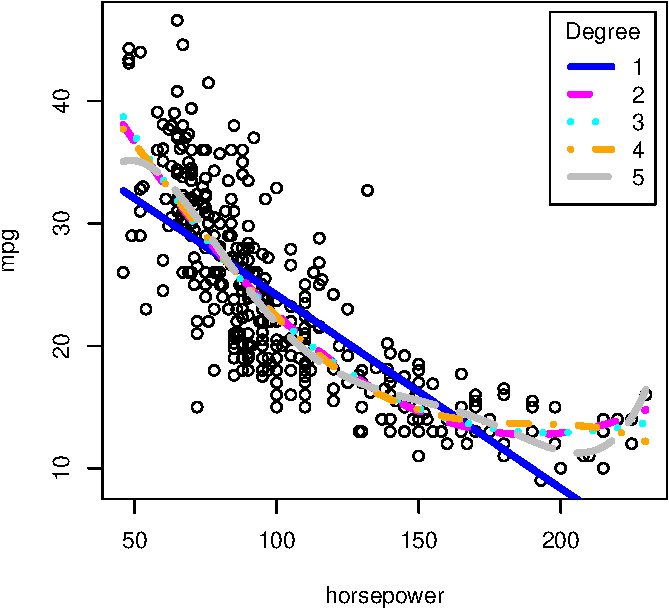
\includegraphics[width=0.5\linewidth]{JSS-article-3_files/figure-latex/mpg-horsepower-scatterplot-polynomials-1} 

}

\caption{\code{mpg} vs. \code{horsepower} for the \code{Auto} data, showing fitted polynomials of degree 1 through 5.}\label{fig:mpg-horsepower-scatterplot-polynomials}
\end{figure}
\end{CodeChunk}

We'll focus here on the relationship of \code{mpg} (miles per gallon) to
\code{horsepower}, as displayed in Figure
\ref{fig:mpg-horsepower-scatterplot-polynomials}. The relationship
between the two variables is monotone, decreasing, and nonlinear.
Following \citet{JamesEtAl:2021}, we'll consider approximating the
relationship by a polynomial regression, with the degree of the
polynomial \(p\) ranging from 1 (a linear regression) to 10.\footnote{Although
  it serves to illustrate the use of CV, a polynomial is not the best
  choice here. Consider, for example the scatterplot for log-transformed
  \texttt{mpg} and \texttt{horsepower}, produced by
  \texttt{plot(mpg\ \textasciitilde{}\ horsepower,\ data=Auto,\ log="xy")}
  (execution of which is left to the reader). We revisit the \code{Auto}
  data in Section \ref{cross-validating-model-specification}.}
Polynomial fits for \(p = 1\) to \(5\) are shown in Figure
\ref{fig:mpg-horsepower-scatterplot-polynomials}. The linear fit is
clearly inappropriate; the fits for \(p = 2\) (quadratic) through \(4\)
are very similar; and the fit for \(p = 5\) may over-fit the data by
chasing one or two relatively high \texttt{mpg} values at the right (but
see the CV results reported below).

Figure \ref{fig:mpg-horsepower-MSE-se} shows two measures of estimated
(squared) error as a function of polynomial-regression degree: The
mean-squared error (``MSE''), defined as
\(\mathsf{MSE} = \frac{1}{n}\sum_{i=1}^n (y_i - \widehat{y}_i)^2\), and
the usual residual variance, defined as
\(\widehat{\sigma}^2 = \frac{1}{n - p - 1} \sum_{i=1}^n (y_i - \widehat{y}_i)^2\).
The former necessarily declines with \(p\) (or, more strictly, can't
increase with \(p\)), while the latter gets slightly larger for the
largest values of \(p\), with the ``best'' value, by a small margin, for
\(p = 7\).

\begin{CodeChunk}
\begin{figure}

{\centering 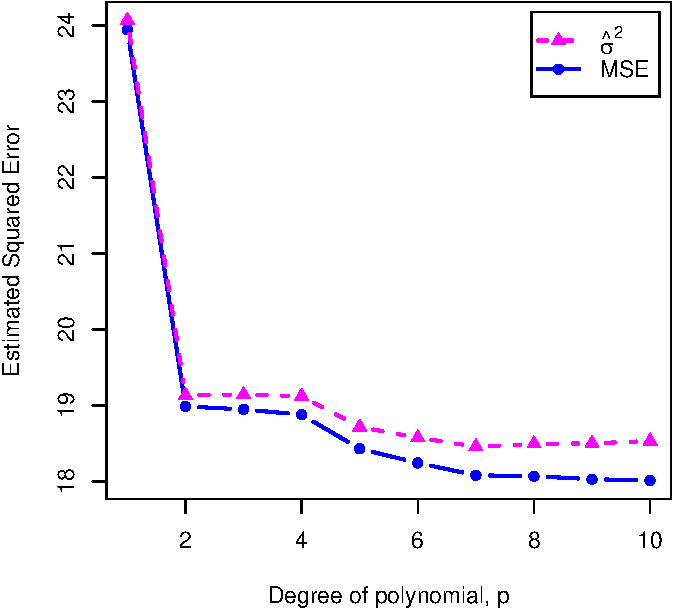
\includegraphics[width=0.5\linewidth]{JSS-article-3_files/figure-latex/mpg-horsepower-MSE-se-1} 

}

\caption[Estimated squared error as a function of polynomial degree, $p$]{Estimated squared error as a function of polynomial degree, $p$}\label{fig:mpg-horsepower-MSE-se}
\end{figure}
\end{CodeChunk}

The generic \texttt{cv()} function has an \texttt{"lm"} method,

\begin{CodeChunk}
\begin{CodeInput}
R> args(cv:::cv.lm)
\end{CodeInput}
\begin{CodeOutput}
function (model, data = insight::get_data(model), criterion = mse, 
    k = 10L, reps = 1L, seed = NULL, details = k <= 10L, confint = n >= 
        400L, level = 0.95, method = c("auto", "hatvalues", "Woodbury", 
        "naive"), ncores = 1L, ...) 
NULL
\end{CodeOutput}
\end{CodeChunk}

which takes the following arguments:

\begin{itemize}
\item
  \code{model}, an \code{"lm"} object, the only required argument.
\item
  \code{data}, which can usually be inferred from the \code{model}
  object.
\item
  \code{criterion}, a function to compute the CV criterion (defaulting
  to \code{mse}).
\item
  \code{k}, the number of folds to employ (defaulting to \code{10}); the
  character value \code{"n"} or \code{"loo"} may be supplied to specify
  leave-one-out cross-validation.
\item
  \code{reps}, the number of times to repeat the CV procedure
  (defaulting to 1).
\item
  \code{seed}, the seed for \proglang{R}'s pseudo-random number
  generator; if not specified a value is randomly selected, reported,
  and saved, so that the CV procedure is replicable.
\item
  \code{confint}, whether or not to compute a confidence interval for
  the CV criterion, defaulting to \code{TRUE} if there are at least 400
  cases; a confidence interval is computed only if the CV criterion can
  be expressed as the average of casewise components (see Section
  \ref{computation-of-the-bias-corrected-cv-criterion-and-confidence-intervals}
  for details).
\item
  \code{level}, the level for the confidence interval (defaulting to
  \code{0.95}).
\item
  \code{method}, the computational method to employ: \code{"hatvalues"}
  is relevant only for LOO CV and bases computation on the hatvalues for
  the linear model; \code{"Woodbury"} employs the Woodbury matrix
  identity to compute the CV criterion with each fold deleted;
  \code{"naive"} updates the model using the \code{update()} function;
  and \code{"auto"} selects \code{"hatvalues"} for LOO CV and
  \code{"Woodbury"} for \(k\)-fold CV, both of which are much more
  efficient than literally updating the least-squares fit (see below and
  Section
  \ref{efficient-computations-for-linear-and-generalized-linear-models}).
\item
  \code{ncores}, the number of cores to employ for parallel computation;
  if \code{cores = 1} (the default), the computations are not
  parallelized.
\end{itemize}

To illustrate, we perform 10-fold CV for a quadratic polynomial fit to
the \code{Auto} data:

\begin{CodeChunk}
\begin{CodeInput}
R> m.auto <- lm(mpg ~ poly(horsepower, 2), data=Auto)
R> summary(m.auto)
\end{CodeInput}
\begin{CodeOutput}

Call:
lm(formula = mpg ~ poly(horsepower, 2), data = Auto)

Residuals:
     Min       1Q   Median       3Q      Max 
-14.7135  -2.5943  -0.0859   2.2868  15.8961 

Coefficients:
                      Estimate Std. Error t value Pr(>|t|)
(Intercept)            23.4459     0.2209  106.13   <2e-16
poly(horsepower, 2)1 -120.1377     4.3739  -27.47   <2e-16
poly(horsepower, 2)2   44.0895     4.3739   10.08   <2e-16

Residual standard error: 4.374 on 389 degrees of freedom
Multiple R-squared:  0.6876,    Adjusted R-squared:  0.686 
F-statistic:   428 on 2 and 389 DF,  p-value: < 2.2e-16
\end{CodeOutput}
\begin{CodeInput}
R> cv(m.auto, confint=TRUE)
\end{CodeInput}
\begin{CodeOutput}
R RNG seed set to 226376
\end{CodeOutput}
\begin{CodeOutput}
10-Fold Cross Validation
method: Woodbury
criterion: mse
cross-validation criterion = 19.33326
bias-adjusted cross-validation criterion = 19.31477
95% CI for bias-adjusted CV criterion = (15.83621, 22.79333)
full-sample criterion = 18.98477 
\end{CodeOutput}
\end{CodeChunk}

The function reports the CV estimate of MSE, a bias-adjusted estimate of
the MSE (the bias adjustment is explained in Section
\ref{computation-of-the-bias-corrected-cv-criterion-and-confidence-intervals}),
and the MSE is also computed for the original, full-sample regression.
Because the number of cases \(n = 392 < 400\) for the \code{Auto} data,
we set the argument \code{confint=TRUE} to obtain a confidence interval
for the MSE, which proves to be quite wide.

To perform LOO CV:

\begin{CodeChunk}
\begin{CodeInput}
R> cv(m.auto, k="loo")
\end{CodeInput}
\begin{CodeOutput}
n-Fold Cross Validation
method: hatvalues
criterion: mse
cross-validation criterion = 19.24821
\end{CodeOutput}
\end{CodeChunk}

The \code{"hatvalues"} method reports only the CV estimate of MSE.
Alternative methods are to use the Woodbury matrix identity or the
``naive'' approach of literally refitting the model with each case
omitted. All three methods produce exact results for a linear model
(within the precision of floating-point computations):

\begin{CodeChunk}
\begin{CodeInput}
R> cv(m.auto, k="loo", method="naive", confint=TRUE)
\end{CodeInput}
\begin{CodeOutput}
n-Fold Cross Validation
method: naive
criterion: mse
cross-validation criterion = 19.24821
bias-adjusted cross-validation criterion = 19.24787
95% CI for bias-adjusted CV criterion = (15.77884, 22.71691)
full-sample criterion = 18.98477 
\end{CodeOutput}
\begin{CodeInput}
R> cv(m.auto, k="loo", method="Woodbury", confint=TRUE)
\end{CodeInput}
\begin{CodeOutput}
n-Fold Cross Validation
method: Woodbury
criterion: mse
cross-validation criterion = 19.24821
bias-adjusted cross-validation criterion = 19.24787
95% CI for bias-adjusted CV criterion = (15.77884, 22.71691)
full-sample criterion = 18.98477 
\end{CodeOutput}
\end{CodeChunk}

The \code{"naive"} and \code{"Woodbury"} methods also return the
bias-adjusted estimate of MSE (and a confidence interval around it)
along with the full-sample MSE, but bias isn't an issue for LOO CV.

This is a small regression problem and all three computational
approaches are essentially instantaneous, but it is still of interest to
investigate their relative speed. In the following comparison, we
include the \code{cv.glm()} function from the \pkg{boot} package, which
takes the naive approach, and for which we have to fit the linear model
as an equivalent Gaussian GLM. We use the \code{microbenchmark()}
function from the package of the same name \citep{Mersmann:2023} for the
timings:

\begin{CodeChunk}
\begin{CodeInput}
R> m.auto.glm <- glm(mpg ~ poly(horsepower, 2), data=Auto)
R> boot::cv.glm(Auto, m.auto.glm)$delta # MSE, biased-corrected MSE
\end{CodeInput}
\begin{CodeOutput}
[1] 19.24821 19.24787
\end{CodeOutput}
\begin{CodeInput}
R> microbenchmark::microbenchmark(
+   hatvalues = cv(m.auto, k="loo"),
+   Woodbury = cv(m.auto, k="loo", method="Woodbury"),
+   naive = cv(m.auto, k="loo", method="naive"),
+   cv.glm = boot::cv.glm(Auto, m.auto.glm),
+   times=10
+ )
\end{CodeInput}
\begin{CodeOutput}
Warning in microbenchmark::microbenchmark(hatvalues = cv(m.auto, k = "loo"), :
less accurate nanosecond times to avoid potential integer overflows
\end{CodeOutput}
\begin{CodeOutput}
Unit: milliseconds
      expr        min         lq       mean     median         uq        max
 hatvalues   1.139062   1.184244   1.202678   1.194248   1.205769   1.297117
  Woodbury  12.106521  12.310701  13.115158  12.337515  12.808810  16.149900
     naive 217.941773 219.491204 225.861284 220.053909 222.015410 278.078974
    cv.glm 373.900074 379.259963 397.907632 382.333036 437.228141 441.112358
 neval
    10
    10
    10
    10
\end{CodeOutput}
\end{CodeChunk}

On our computer, using the hatvalues is about an order of magnitude
faster than employing Woodbury matrix updates, and more than two orders
of magnitude faster than refitting the model.

\subsection{Comparing competing
models}\label{comparing-competing-models}

The \code{cv()} function also has a method that can be applied to a list
of regression models for the same data, composed using the
\code{models()} function. For \(k\)-fold CV, the same folds are used for
the competing models, which reduces random error in their comparison.
This result can also be obtained by specifying a common seed for
\proglang{R}'s random-number generator while applying \code{cv()}
separately to each model, but employing a list of models is more
convenient for both \(k\)-fold and LOO CV (where there is no random
component to the composition of the \(n\) folds).

We illustrate with the polynomial regression models of varying degree
for the \code{Auto} data, beginning by fitting and saving the 10 models:

\begin{CodeChunk}
\begin{CodeInput}
R> mlist <- vector(10, mode="list")
R> for (p in 1:10) mlist[[p]] <- lm(mpg ~ poly(horsepower, p), data = Auto)
R> names(mlist) <- paste0("m.", 1:10)
R> mlist[2] # e.g., the quadratic fit
\end{CodeInput}
\begin{CodeOutput}
$m.2

Call:
lm(formula = mpg ~ poly(horsepower, p), data = Auto)

Coefficients:
         (Intercept)  poly(horsepower, p)1  poly(horsepower, p)2  
               23.45               -120.14                 44.09  
\end{CodeOutput}
\end{CodeChunk}

We then apply \code{cv()} to the list of 10 models (the \code{data}
argument is required):

\begin{CodeChunk}
\begin{CodeInput}
R> # 10-fold CV
R> mlist <- do.call(models, mlist) # create "modList" object
R> 
R> cv.auto.10 <- cv(mlist, data=Auto, seed=2120)
R> cv.auto.10[2] # e.g., for quadratic model
\end{CodeInput}
\begin{CodeOutput}

Model m.2:
10-Fold Cross Validation
method: Woodbury
cross-validation criterion = 19.34601
bias-adjusted cross-validation criterion = 19.32699
full-sample criterion = 18.98477 
\end{CodeOutput}
\begin{CodeInput}
R> # LOO CV
R> cv.auto.loo <- cv(mlist, data=Auto, k="loo")
R> cv.auto.loo[2] # e.g., for quadratic model
\end{CodeInput}
\begin{CodeOutput}

Model m.2:
n-Fold Cross Validation
method: hatvalues
cross-validation criterion = 19.24821
\end{CodeOutput}
\end{CodeChunk}

The \code{models()} function takes an arbitrary number of regression
models as its arguments, which are optionally named, to create a
\code{"modList"} object. Because we generated the polynomial regression
models in a named list, we conveniently employ \code{do.call()} to
supply the models as arguments to \code{models()}. The names created for
the list (e.g., \code{"m.2"}) are then used for the models. We can also
invoke the \code{plot()} method for \code{"cvModList"} objects to
compare the models (see Figure
\ref{fig:polynomial-regression-CV-graph-2}):

\begin{CodeChunk}
\begin{CodeInput}
R> plot(cv.auto.10, main="Polynomial Regressions, 10-Fold CV",
+      axis.args=list(labels=1:10), xlab="Degree of Polynomial, p")
R> plot(cv.auto.loo, main="Polynomial Regressions, LOO CV",
+      axis.args=list(labels=1:10), xlab="Degree of Polynomial, p")
\end{CodeInput}
\begin{figure}

{\centering \subfloat[\label{fig:polynomial-regression-CV-graph-2-1}]{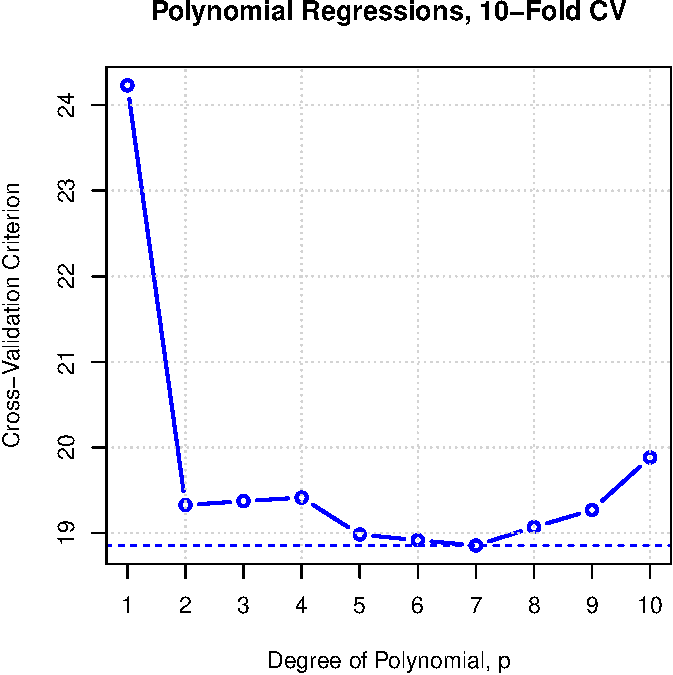
\includegraphics[width=0.5\linewidth]{JSS-article-3_files/figure-latex/polynomial-regression-CV-graph-2-1} }\subfloat[\label{fig:polynomial-regression-CV-graph-2-2}]{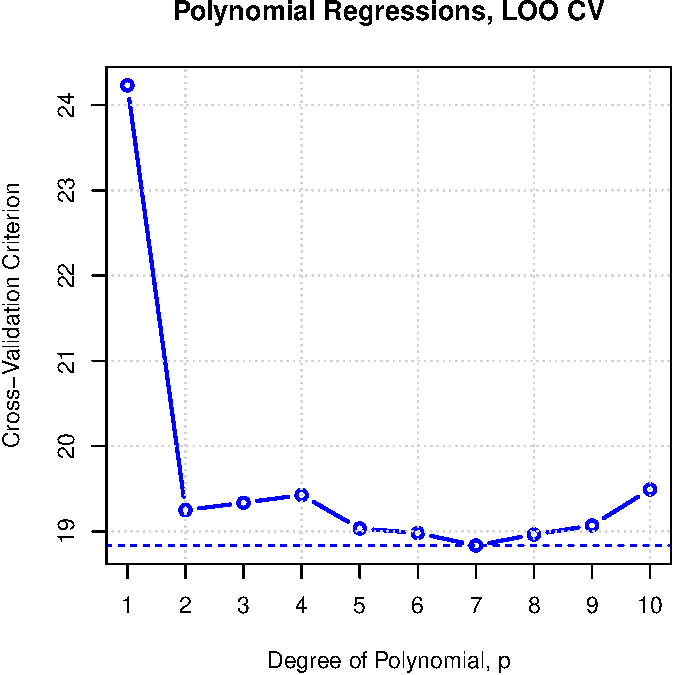
\includegraphics[width=0.5\linewidth]{JSS-article-3_files/figure-latex/polynomial-regression-CV-graph-2-2} }

}

\caption[Cross-validated (a) 10-fold and (b) LOO MSE as a function of polynomial degree, $p$]{Cross-validated (a) 10-fold and (b) LOO MSE as a function of polynomial degree, $p$.}\label{fig:polynomial-regression-CV-graph-2}
\end{figure}
\end{CodeChunk}

In this example, 10-fold and LOO CV produce generally similar results,
and also results that are similar to those produced by the estimated
error variance \(\widehat{\sigma}^2\) for each model (cf., Figure
\ref{fig:mpg-horsepower-MSE-se} on page
\pageref{fig:mpg-horsepower-MSE-se}), except for the highest-degree
polynomials, where the CV results more clearly suggest over-fitting.

\section{Cross-validating mixed-effects
models}\label{cross-validating-mixed-effects-models}

The fundamental analogy for cross-validation is to the collection of new
data. That is, predicting the response in each fold from the model fit
to data in the other folds is like using the model fit to all of the
data to predict the response for new cases from the values of the
predictors for those new cases. As we explained, the application of this
idea to independently sampled cases is straightforward.

In contrast, mixed-effects models are fit to \emph{dependent} data, in
which cases are clustered, such as hierarchical data, where the clusters
comprise higher-level units (e.g., students clustered in schools), or
longitudinal data, where the clusters are individuals and the cases are
repeated observations on the individuals over time.\footnote{There are,
  however, more complex situations that give rise to so-called
  \emph{crossed} (rather than \emph{nested}) random effects. For
  example, consider students within classes within schools. In primary
  schools, students typically are in a single class, and so classes are
  nested within schools. In secondary schools, however, students
  typically take several classes and students who are together in a
  particular class may not be together in other classes; consequently,
  random effects based on classes within schools are crossed. The
  \code{lmer()} function in the \pkg{lme4} package, for example, is
  capable of modeling both nested and crossed random effects, and the
  \code{cv()} methods for mixed models in the \pkg{cv} package pertain
  to both nested and crossed random effects. We present an example of
  the latter in a vignette for the \pkg{cv} package.}

We can think of two approaches to applying cross-validation to clustered
data:\footnote{We subsequently discovered that \citet[Section
  8]{Vehtari:2023} makes similar points.}

\begin{enumerate}
\def\labelenumi{\arabic{enumi}.}
\item
  Treat CV as analogous to predicting the response for one or more cases
  in a \emph{newly observed cluster}. In this instance, the folds
  comprise one or more whole clusters; we refit the model with all of
  the cases in clusters in the current fold removed; and then we predict
  the response for the cases in clusters in the current fold. These
  predictions are based only on fixed effects because the random effects
  for the omitted clusters are construed to be unknown, as they would be
  for data on cases in newly observed clusters.
\item
  Treat CV as analogous to predicting the response for a newly observed
  case in an \emph{existing cluster}. In this instance, the folds
  comprise one or more individual cases, and the predictions can use
  both the fixed and random effects---so-called ``best-linear-unbiased
  predictors'' or ``BLUPs.''
\end{enumerate}

\subsection{Example: The High-School and Beyond
data}\label{example-the-high-school-and-beyond-data}

Following their use by \citet{RaudenbushBryk:2002}, data from the 1982
\emph{High School and Beyond} (HSB) survey have become a staple of the
literature on mixed-effects models. The HSB data are used by \citet[Sec.
7.2.2]{FoxWeisberg:2019} to illustrate the application of linear mixed
models to hierarchical data, and we'll closely follow their example
here.

The HSB data are included in the \code{MathAchieve} and
\code{MathAchSchool} data sets in the \pkg{nlme} package
\citep{PinheiroBates:2000}. \code{MathAchieve} comprises
individual-level data on 7185 students in 160 high schools, and
\code{MathAchSchool} contains school-level data:

\begin{CodeChunk}
\begin{CodeInput}
R> data("MathAchieve", package="nlme")
R> dim(MathAchieve)
\end{CodeInput}
\begin{CodeOutput}
[1] 7185    6
\end{CodeOutput}
\begin{CodeInput}
R> head(MathAchieve, 3)
\end{CodeInput}
\begin{CodeOutput}
Grouped Data: MathAch ~ SES | School
  School Minority    Sex    SES MathAch MEANSES
1   1224       No Female -1.528   5.876  -0.428
2   1224       No Female -0.588  19.708  -0.428
3   1224       No   Male -0.528  20.349  -0.428
\end{CodeOutput}
\begin{CodeInput}
R> tail(MathAchieve, 3)
\end{CodeInput}
\begin{CodeOutput}
Grouped Data: MathAch ~ SES | School
     School Minority    Sex    SES MathAch MEANSES
7183   9586       No Female  1.332  19.641   0.627
7184   9586       No Female -0.008  16.241   0.627
7185   9586       No Female  0.792  22.733   0.627
\end{CodeOutput}
\begin{CodeInput}
R> data("MathAchSchool", package="nlme")
R> dim(MathAchSchool)
\end{CodeInput}
\begin{CodeOutput}
[1] 160   7
\end{CodeOutput}
\begin{CodeInput}
R> head(MathAchSchool, 2)
\end{CodeInput}
\begin{CodeOutput}
     School Size Sector PRACAD DISCLIM HIMINTY MEANSES
1224   1224  842 Public   0.35   1.597       0  -0.428
1288   1288 1855 Public   0.27   0.174       0   0.128
\end{CodeOutput}
\begin{CodeInput}
R> tail(MathAchSchool, 2)
\end{CodeInput}
\begin{CodeOutput}
     School Size   Sector PRACAD DISCLIM HIMINTY MEANSES
9550   9550 1532   Public   0.45   0.791       0   0.059
9586   9586  262 Catholic   1.00  -2.416       0   0.627
\end{CodeOutput}
\end{CodeChunk}

The first few students are in school number 1224 and the last few in
school 9586.

We'll use only the \code{School}, \code{SES} (students' socioeconomic
status), and \code{MathAch} (their score on a standardized
math-achievement test) variables in the \code{MathAchieve} data set, and
\code{Sector} (\code{"Catholic"} or \code{"Public"}) in the
\code{MathAchSchool} data set.

Some data-management is required before fitting a mixed-effects model to
the HSB data:

\begin{CodeChunk}
\begin{CodeInput}
R> HSB <- MathAchieve
R> HSB <- merge(MathAchSchool[, c("School", "Sector")],
+              HSB[, c("School", "SES", "MathAch")], by="School")
R> names(HSB) <- tolower(names(HSB))
R> HSB <- within(HSB, {
+   mean.ses <- ave(ses, school)
+   cses <- ses - mean.ses
+ })
\end{CodeInput}
\end{CodeChunk}

In the process, we merge variables from the school-level and
student-level data sets, and create two new school-level variables:
\code{mean.ses}, which is the average SES for students in each school;
and \code{cses}, which is the individual students' SES centered at their
school means. For details, see \citet[Sec. 7.2.2]{FoxWeisberg:2019}.

Still following Fox and Weisberg, we proceed to use the \code{lmer()}
function in the \pkg{lme4} package \citep{BatesEtAl:2015} to fit a mixed
model for math achievement to the HSB data:

\begin{CodeChunk}
\begin{CodeInput}
R> library("lme4", quietly=TRUE)
R> hsb.lmer <- lmer(mathach ~ mean.ses*cses + sector*cses
+                    + (cses | school), data=HSB)
R> summary(hsb.lmer, correlation=FALSE)
\end{CodeInput}
\begin{CodeOutput}
Linear mixed model fit by REML ['lmerMod']
Formula: mathach ~ mean.ses * cses + sector * cses + (cses | school)
   Data: HSB

REML criterion at convergence: 46503.7

Scaled residuals: 
     Min       1Q   Median       3Q      Max 
-3.15926 -0.72319  0.01704  0.75444  2.95822 

Random effects:
 Groups   Name        Variance Std.Dev. Corr
 school   (Intercept)  2.380   1.5426       
          cses         0.101   0.3179   0.39
 Residual             36.721   6.0598       
Number of obs: 7185, groups:  school, 160

Fixed effects:
                    Estimate Std. Error t value
(Intercept)          12.1279     0.1993  60.856
mean.ses              5.3329     0.3692  14.446
cses                  2.9450     0.1556  18.928
sectorCatholic        1.2266     0.3063   4.005
mean.ses:cses         1.0393     0.2989   3.477
cses:sectorCatholic  -1.6427     0.2398  -6.851
\end{CodeOutput}
\end{CodeChunk}

We can then cross-validate at the cluster (i.e., school) level,

\begin{CodeChunk}
\begin{CodeInput}
R> cv(hsb.lmer, k=10, clusterVariables="school", seed=5240)
\end{CodeInput}
\begin{CodeOutput}
R RNG seed set to 5240
\end{CodeOutput}
\begin{CodeOutput}
10-Fold Cross Validation based on 160 {school} clusters
criterion: mse
cross-validation criterion = 39.15662
bias-adjusted cross-validation criterion = 39.14844
95% CI for bias-adjusted CV criterion = (38.06554, 40.23135)
full-sample criterion = 39.00599 
\end{CodeOutput}
\end{CodeChunk}

or at the case (i.e., student) level,

\begin{CodeChunk}
\begin{CodeInput}
R> cv(hsb.lmer, seed=1575)
\end{CodeInput}
\begin{CodeOutput}
R RNG seed set to 1575
\end{CodeOutput}
\begin{CodeOutput}
Warning in checkConv(attr(opt, "derivs"), opt$par, ctrl = control$checkConv, :
Model failed to converge with max|grad| = 0.00587207 (tol = 0.002, component 1)
\end{CodeOutput}
\begin{CodeOutput}
boundary (singular) fit: see help('isSingular')
\end{CodeOutput}
\begin{CodeOutput}
10-Fold Cross Validation
criterion: mse
cross-validation criterion = 37.44473
bias-adjusted cross-validation criterion = 37.33801
95% CI for bias-adjusted CV criterion = (36.28761, 38.38841)
full-sample criterion = 36.06767 
\end{CodeOutput}
\end{CodeChunk}

For cluster-level CV, the \code{clusterVariables} argument tells
\code{cv()} how the clusters are defined. Were there more than one
clustering variable, say classes within schools, these would be provided
as a character vector of variable names:
\code{clusterVariables = c("school", "class")}. For cluster-level CV,
the default is \code{k = "loo"}, that is, leave one cluster out at a
time; we instead specify \code{k = 10} folds of clusters, each fold
therefore comprising \(160/10 = 16\) schools.

If the \code{clusterVariables} argument is omitted, then case-level CV
is employed, with \code{k = 10} folds as the default, here each with
\(7185/10 \approx 719\) students. Notice that one of the 10 models refit
with a fold removed failed to converge. Convergence problems are common
in mixed-effects modeling. The issue here is that an estimated variance
component is close to or equal to 0, which is at a boundary of the
parameter space. That shouldn't disqualify the fitted model for the kind
of prediction required for cross-validation.

\code{cv()} also has methods for mixed models fit by the \code{glmer()}
function in the \pkg{lme4} package, the \code{lme()} function in the
\pkg{nlme} package \citep{PinheiroBates:2000}, and the \code{glmmTMB()}
function in the \pkg{glmmTMB} package \citep{BrooksEtAl}, along with a
simple procedure for extending \code{cv()} to other classes of
mixed-effects models. See the vignettes in the \pkg{cv} package for
details.

\subsection{Example: Contrasting cluster-based and case-based
CV}\label{example-contrasting-cluster-based-and-case-based-cv}

In this section, we introduce an artificial data set that exemplifies
aspects of cross-validation particular to hierarchical models. Using
this data set, we show that model comparisons employing cluster-based
and those employing case-based cross-validation may not agree on a
``best'' model. Furthermore, commonly used measures of fit, such as
mean-squared error, do not necessarily become smaller as models become
larger, even when the models are nested, and even when the measure of
fit is computed for the whole data set.

Consider a researcher studying improvement in a skill, singing, for
example, among students enrolled in a four-year voice program at a music
conservatory. The plan is to measure each student's skill level at the
beginning of the program and every year thereafter until the end of the
program, resulting in 5 annual measurements for each student. It turns
out that singing appeals to students of all ages, and students enrolling
in the program range in age from 20 to 70. Moreover, participants'
untrained singing skill is similar at all ages, as is their rate of
progress with training. All students complete the four-year program.

The researcher, who has more expertise in singing than in modeling,
decides to model the response, \(y\), singing skill, as a function of
age, \(x\), reasoning that students get older during their stay in the
program, and (incorrectly) that age can serve as a proxy for elapsed
time. The researcher knows that a mixed model should be used to account
for clustering due to the expected similarity of measurements taken from
each student.

We start by generating the data, using parameters consistent with the
description above and meant to highlight the issues that arise in
cross-validating mixed-effects models:\footnote{We invite the interested
  reader to experiment with varying the parameters of our example.}

\begin{CodeChunk}
\begin{CodeInput}
R> # Parameters:
R> set.seed(9693) 
R> Nb <- 100     # number of groups
R> Nw <- 5       # number of individuals within groups
R> Bb <- 0       # between-group regression coefficient on group mean
R> SDre <- 2.0   # between-group SD of random level relative to group mean of x
R> SDwithin <- 0.5  # within group SD
R> Bw <- 1          # within group effect of x
R> Ay <- 10         # intercept for response
R> Ax <- 20         # starting level of x
R> Nx <- Nw*10      # number of distinct x values
R> 
R> Data <- data.frame(
+   group = factor(rep(1:Nb, each=Nw)),
+   x = Ax + rep(1:Nx, length.out = Nw*Nb)
+ ) |> within ({
+   xm  <- ave(x, group, FUN = mean) # within-group mean
+   y <- Ay +
+     Bb * xm +                    # contextual effect
+     Bw * (x - xm) +              # within-group effect
+     rnorm(Nb, sd=SDre)[group] +  # random level by group
+     rnorm(Nb*Nw, sd=SDwithin)    # random error within groups
+ })
\end{CodeInput}
\end{CodeChunk}

Figure \ref{fig:plot1} (a) shows a scatterplot the data for a
representative group of 10 (without loss of generality, the first 10) of
the 100 students, displaying the 95\% concentration ellipse for each
cluster.

\begin{CodeChunk}
\begin{figure}

{\centering \subfloat[\label{fig:plot1-1}]{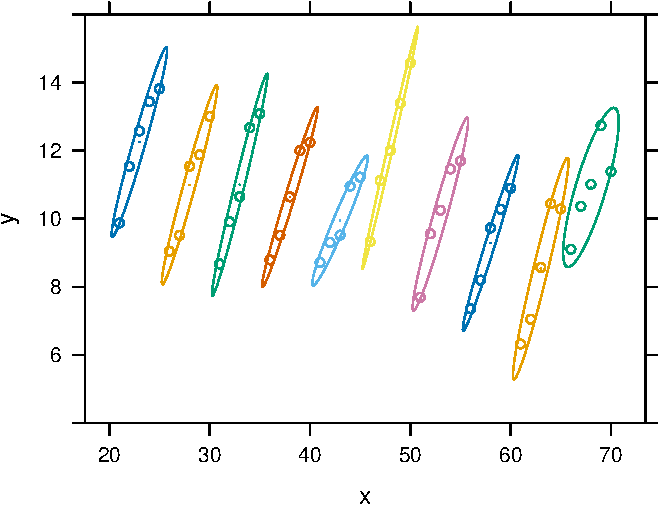
\includegraphics[width=0.45\linewidth]{JSS-article-3_files/figure-latex/plot1-1} }\subfloat[\label{fig:plot1-2}]{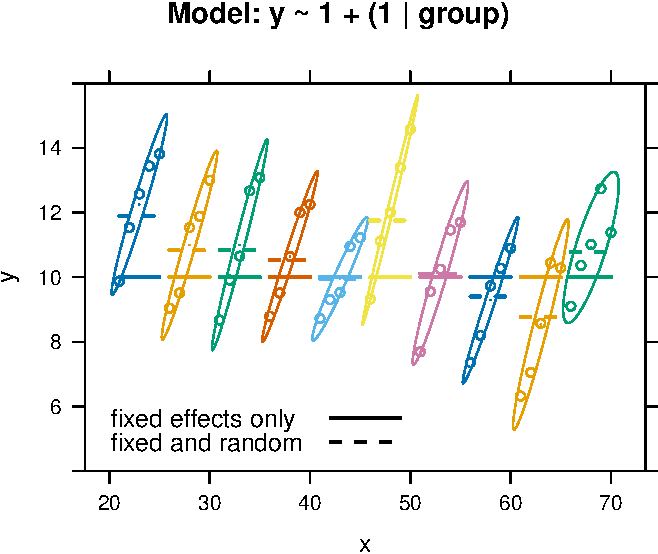
\includegraphics[width=0.45\linewidth]{JSS-article-3_files/figure-latex/plot1-2} }\newline\subfloat[\label{fig:plot1-3}]{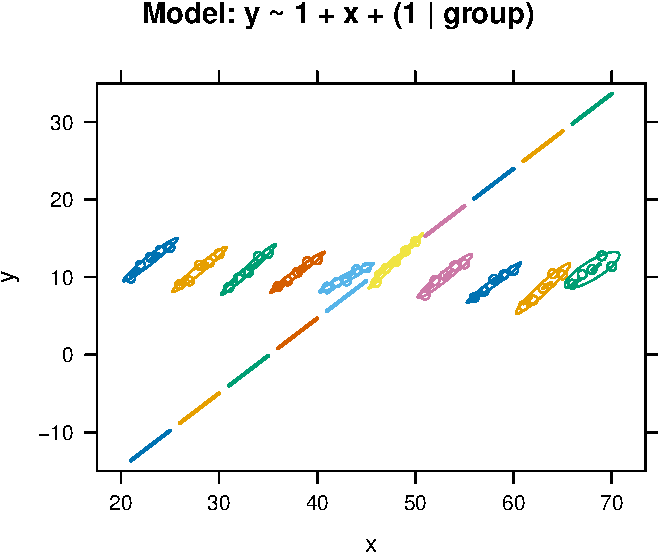
\includegraphics[width=0.45\linewidth]{JSS-article-3_files/figure-latex/plot1-3} }\subfloat[\label{fig:plot1-4}]{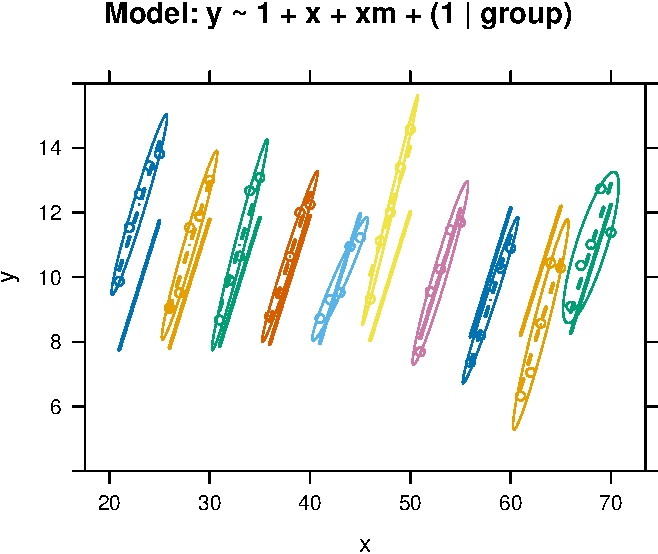
\includegraphics[width=0.45\linewidth]{JSS-article-3_files/figure-latex/plot1-4} }\newline\subfloat[\label{fig:plot1-5}]{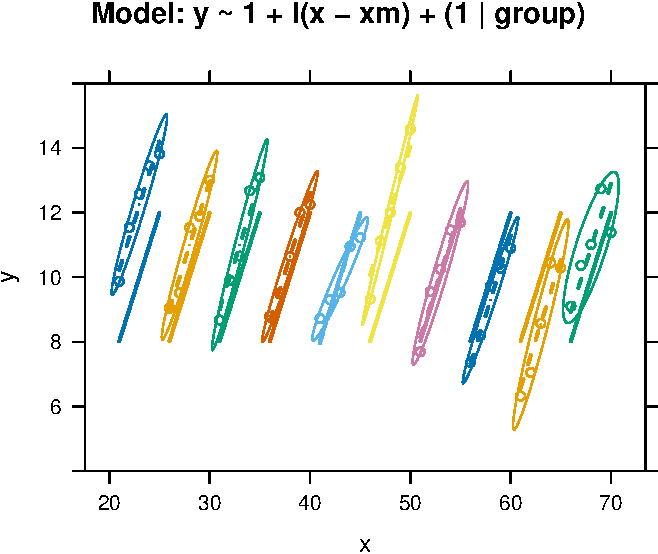
\includegraphics[width=0.45\linewidth]{JSS-article-3_files/figure-latex/plot1-5} }

}

\caption[(a) Hierarchical data set, showing the first 10 of 100 students, and (b)--(e) predictions from several mixed models fit to the data]{(a) Hierarchical data set, showing the first 10 of 100 students, and (b)--(e) predictions from several mixed models fit to the data}\label{fig:plot1}
\end{figure}
\end{CodeChunk}

The between-student effect of age is 0 but the within-student effect is
1. Due to the large variation in ages between students, the
least-squares regression of singing skill on age (for the 500
observations among all 100 students) produces an estimated slope close
to 0 (though with a small \(p\)-value), because the slope is heavily
weighted toward the between-student effect:

\begin{CodeChunk}
\begin{CodeInput}
R> summary(lm(y ~ x, data=Data))
\end{CodeInput}
\begin{CodeOutput}

Call:
lm(formula = y ~ x, data = Data)

Residuals:
    Min      1Q  Median      3Q     Max 
-5.7713 -1.6583 -0.0894  1.5520  7.6240 

Coefficients:
            Estimate Std. Error t value Pr(>|t|)
(Intercept) 9.050430   0.347189  26.068  < 2e-16
x           0.020908   0.007273   2.875  0.00422

Residual standard error: 2.347 on 498 degrees of freedom
Multiple R-squared:  0.01632,   Adjusted R-squared:  0.01435 
F-statistic: 8.263 on 1 and 498 DF,  p-value: 0.004219
\end{CodeOutput}
\end{CodeChunk}

We proceed to fit several mixed-effects models to the data, using the
\texttt{compareCoefs()} function from the \pkg{car} package
\citep{FoxWeisberg:2019} to display the fixed-effect estimates for these
models. We discuss each of these models below.

\begin{CodeChunk}
\begin{CodeInput}
R> mod.0 <- lmer(y ~ 1 + (1 | group), Data)
R> mod.1 <- lmer(y ~ x + (1 | group), Data)
R> mod.2 <- lmer(y ~ x + xm + (1 | group), Data)
R> mod.3 <- lmer(y ~ I(x - xm) + (1 | group), Data)
R> library("car", quietly=TRUE)
R> compareCoefs(mod.0, mod.1, mod.2, mod.3)
\end{CodeInput}
\begin{CodeOutput}
Calls:
1: lmer(formula = y ~ 1 + (1 | group), data = Data)
2: lmer(formula = y ~ x + (1 | group), data = Data)
3: lmer(formula = y ~ x + xm + (1 | group), data = Data)
4: lmer(formula = y ~ I(x - xm) + (1 | group), data = Data)

            Model 1 Model 2 Model 3 Model 4
(Intercept)  10.002 -33.919   9.479  10.002
SE            0.186   1.564   0.617   0.186
                                           
x                    0.9653  0.9915        
SE                   0.0158  0.0160        
                                           
xm                          -0.9800        
SE                           0.0206        
                                           
I(x - xm)                             0.992
SE                                    0.016
                                           
\end{CodeOutput}
\end{CodeChunk}

The initial mixed-effects model, \code{mod.0}, is a simple
random-intercepts model. We obtain predictions from this model for the
fixed effects alone, as would be used for cross-validation based on
clusters (i.e., students), and for fixed and random effects---the
BLUPs---as would be used for cross-validation based on cases (i.e.,
occasions within students). Predictions from \code{mod.0} for the first
10 students are shown in Figure \ref{fig:plot1} (b). The fixed-effect
predictions for the various individuals are identical---the estimated
fixed-effects intercept or estimated general mean of \(y\)---while the
BLUPs are the sums of the fixed-effects intercept and the random
intercepts, and are only slightly shrunken towards the general mean.
Because in our artificial data there is no population relationship
between age and skill, the fixed-effect-only predictions and the BLUPs
are not very different.

Our next model, \code{mod.1}, includes a fixed intercept and the fixed
effect of \code{x}, along with a random intercept. Predictions from this
model appear in Figure \ref{fig:plot1} (c). The BLUPs fit the observed
data very closely, but predictions based on the fixed effects alone,
with a common intercept and slope for all clusters, are very
poor---indeed, much worse than the fixed-effects-only predictions based
on the simpler random-intercept model, \code{mod.0}. We therefore
anticipate (and show later in this section) that case-based
cross-validation will prefer \code{mod.1} to \code{mod.0}, but that
cluster-based cross-validation will prefer \code{mod.0} to \code{mod.1}.

Our third model, \code{mod.2}, includes the ``contextual effect'' of
\(x\)---that is, the cluster mean \code{xm}---along with \(x\) and the
intercept in the fixed-effect part of the model, and a random intercept.
This model is equivalent to fitting
\code{y ~ I(x - xm) + xm + (1 | group)}, which is the model that
generated the data once the coefficient of the contextual predictor
\code{xm} is set to 0 (as it is in \code{mod.3}, discussed below).

Predictions from \code{mod.2} appear in Figure \ref{fig:plot1} (d).
Depending on the estimated variance parameters of the model, a mixed
model like \code{mod.2} will apply varying degrees of shrinkage to the
random-intercept BLUPs that correspond to variation in the heights of
the parallel fitted lines for the individual students. In our contrived
data, \code{mod.2} applies little shrinkage, allowing substantial
variability in the heights of the fitted lines, which closely approach
the observed values for each student. The fit of the mixed model
\code{mod.2} is consequently similar to that of a fixed-effects model
with age and a categorical predictor for individual students (i.e.,
treating students as a factor, and not shown here).

The mixed model \code{mod.2} therefore fits the individual observations
well, and we anticipate a favorable assessment using individual-based
cross-validation. In contrast, the large variability in the BLUPs
results in larger residuals for predictions based on fixed effects
alone, and so we expect that cluster-based cross-validation won't show
an advantage for \code{mod.2} compared to the smaller \code{mod.0},
which includes only fixed and random intercepts.

Had the mixed model applied considerable shrinkage, then neither
cluster-based nor case-based cross-validation would show much
improvement over the random-intercept-only model. In our experience, the
degree of shrinkage does not vary smoothly as parameters are changed but
tends to be ``all or nothing,'' and near the tipping point, the behavior
of estimates can be affected considerably by the choice of algorithm
used to fit the model.

Finally, \code{mod.3} directly estimates the model used to generate the
data. As mentioned, it is a constrained version of \code{mod.2}, with
the coefficient of \code{xm} set to 0, and with \code{x} expressed as a
deviation from the cluster mean \code{xm}. The predictions from
\code{mod.3}, shown in Figure \ref{fig:plot1} (e), are therefore similar
to those from \code{mod.2}.

We next carry out case-based cross-validation, which, as we have
explained, includes both fixed and predicted random effects (i.e.,
BLUPs), and cluster-based cross-validation, which includes fixed effects
only. In order to reduce between-model random variability in comparisons
of models, we apply \code{cv()} to the list of models created by the
\code{models()} function (introduced previously), performing
cross-validation with the same folds for each model (see Figure
\ref{fig:cross-validation-clusters}):

\begin{CodeChunk}
\begin{CodeInput}
R> modlist <- models("~ 1"=mod.0, "~ 1 + x"=mod.1, 
+                   "~ 1 + x + xm"=mod.2, "~ 1 + I(x - xm)"=mod.3)
R> 
R> cvs_clusters <- cv(modlist, data=Data, cluster="group", k=10, seed=6449)
R> plot(cvs_clusters, main="Model Comparison, Cluster-Based CV")
R> 
R> cvs_cases <- cv(modlist, data=Data, seed=9693)
R> plot(cvs_cases, main="Model Comparison, Case-Based CV")
\end{CodeInput}
\begin{figure}

{\centering \subfloat[\label{fig:cross-validation-clusters-1}]{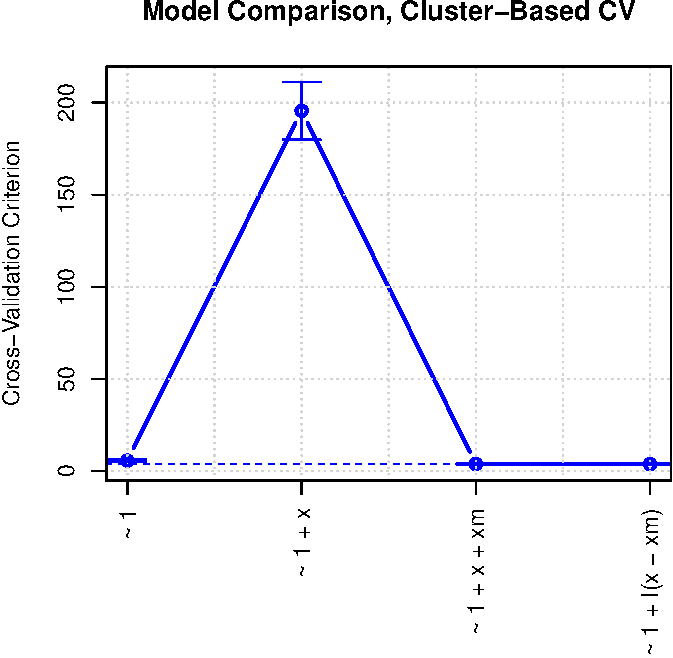
\includegraphics[width=0.45\linewidth]{JSS-article-3_files/figure-latex/cross-validation-clusters-1} }\subfloat[\label{fig:cross-validation-clusters-2}]{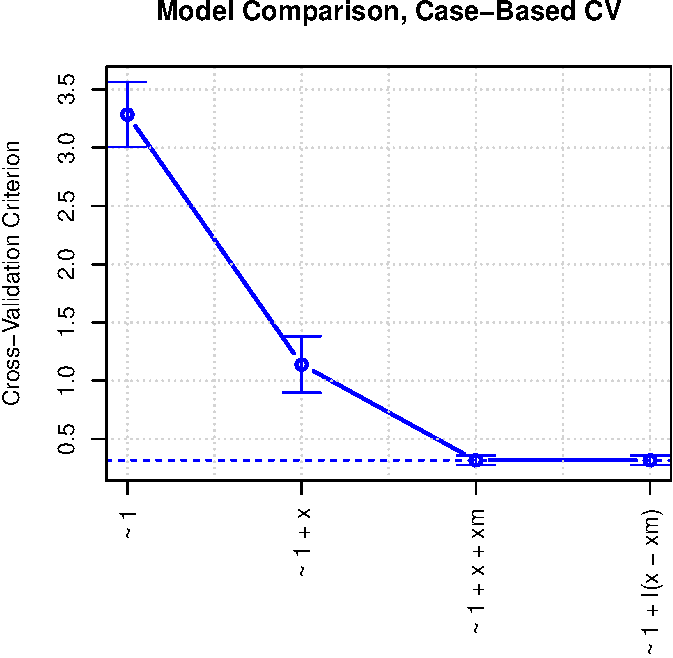
\includegraphics[width=0.45\linewidth]{JSS-article-3_files/figure-latex/cross-validation-clusters-2} }

}

\caption[10-fold (a) cluster-based and (b) case-based cross-validation comparing random intercept models with varying fixed effects]{10-fold (a) cluster-based and (b) case-based cross-validation comparing random intercept models with varying fixed effects. The error bars show the 95\% confidence interval around the CV estimate of the MSE for each model.}\label{fig:cross-validation-clusters}
\end{figure}
\end{CodeChunk}

In summary, \code{mod.1}, with \(x\) alone and without the contextual
mean of \(x\), is assessed as fitting very poorly by cluster-based CV,
but relatively much better by case-based CV. \code{mod.2}, which
includes both \(x\) and its contextual mean, produces better results
using both cluster-based and case-based CV. The data-generating model,
\code{mod.3}, which includes the fixed effect of \code{x - xm} in place
of separate terms in \code{x} and \code{xm}, isn't distinguishable from
\code{mod.2}, which includes \code{x} and \code{xm} separately, even
though \code{mod.2} has an unnecessary parameter (recall that the
population coefficient of \code{xm} is 0 when \code{x} is expressed as
deviations from the contextual mean). These conclusions are consistent
with our observations based on graphing predictions from the various
models in Figure \ref{fig:plot1} (on page \pageref{fig:plot1}), and they
illustrate the desirability of assessing mixed-effect models at
different hierarchical levels.

\section{Cross-validating model
specification}\label{cross-validating-model-specification}

As \citet[Sec. 7.10.2: ``The Wrong and Right Way to Do
Cross-validation'']{HastieTibshiraniFriedman:2009} explain, if the whole
data are used to specify or fine-tune a statistical model, then
subsequent cross-validation of the model is intrinsically misleading,
because the model is selected to fit the whole data, including the part
of the data that remains when each fold is removed. Statistical modeling
is partly a craft, and one could imagine applying that craft to
successive partial data sets, each with a fold removed. The resulting
procedure would be tedious, though possibly worth the effort, but it
would also be difficult to realize in practice: After all, we can hardly
erase our memory of statistical modeling choices between analyzing
partial data sets. Alternatively, if we're able to automate the process
of model specification, then we can more realistically apply CV
mechanically.

The \code{"function"} method for \code{cv()} cross-validates a
model-specification process in a general manner. Functions for four such
model-specification processes are included in the package:
\code{selectStepAIC()}, based on the \code{stepAIC()} function in the
\pkg{MASS} package \citep{VenablesRipley:2002}, performs stepwise
predictor selection for regression models; \code{selectTrans()}, based
on the \code{powerTransform()} function in the \pkg{car} package
\citep{FoxWeisberg:2019}, transforms predictors and the response in a
regression model towards normality; \code{selectTransAndStepAIC()}---the
use of which we illustrate in the current section---performs both of
these procedures sequentially; and \code{selectModelList()}---also
illustrated in the current section---uses CV both to select one of
several competing models, and then, recursively, to estimate prediction
error for the selected model. In a vignette on extending the \pkg{cv}
package, we explain how to specify additional model-selection
procedures.

\subsection{Example: Data transformation and predictor selection for the
Auto
data}\label{example-data-transformation-and-predictor-selection-for-the-auto-data}

To illustrate cross-validation of model specification, we return to the
\code{Auto} data set:\footnote{This example benefits from an email
  conversation with Bill Venables, who of course isn't responsible for
  the use to which we've put his insightful remarks.}

\begin{CodeChunk}
\begin{CodeInput}
R> names(Auto)
\end{CodeInput}
\begin{CodeOutput}
[1] "mpg"          "cylinders"    "displacement" "horsepower"   "weight"      
[6] "acceleration" "year"         "origin"       "name"        
\end{CodeOutput}
\begin{CodeInput}
R> xtabs(~ year, data=Auto)
\end{CodeInput}
\begin{CodeOutput}
year
70 71 72 73 74 75 76 77 78 79 80 81 82 
29 27 28 40 26 30 34 28 36 29 27 28 30 
\end{CodeOutput}
\begin{CodeInput}
R> xtabs(~ origin, data=Auto)
\end{CodeInput}
\begin{CodeOutput}
origin
  1   2   3 
245  68  79 
\end{CodeOutput}
\begin{CodeInput}
R> xtabs(~ cylinders, data=Auto)
\end{CodeInput}
\begin{CodeOutput}
cylinders
  3   4   5   6   8 
  4 199   3  83 103 
\end{CodeOutput}
\end{CodeChunk}

The \code{Auto} data appeared in a preliminary example in Section
\ref{preliminary-example-polynomial-regression}, where we employed CV to
inform the selection of the degree of a polynomial regression of
\code{mpg} on \code{horsepower}. Here, we consider more generally the
problem of predicting \code{mpg} from the other variables in the
\code{Auto} data. We begin with a bit of data management, and then
examine the pairwise relationships among the numeric variables in the
data set (Figure \ref{fig:Auto-explore}, produced by the
\code{scatterplotMatrix()} function in the \pkg{car} package):

\begin{CodeChunk}
\begin{CodeInput}
R> Auto$cylinders <- factor(Auto$cylinders,
+                          labels=c("3-4", "3-4", "5-6", "5-6", "8"))
R> Auto$year <- as.factor(Auto$year)
R> Auto$origin <- factor(Auto$origin,
+                       labels=c("America", "Europe", "Japan"))
R> rownames(Auto) <- make.names(Auto$name, unique=TRUE)
R> Auto$name <- NULL
R> 
R> scatterplotMatrix(~ mpg + displacement + horsepower + weight + acceleration, 
+                   smooth=list(spread=FALSE), data=Auto, pch=".")
\end{CodeInput}
\begin{figure}

{\centering 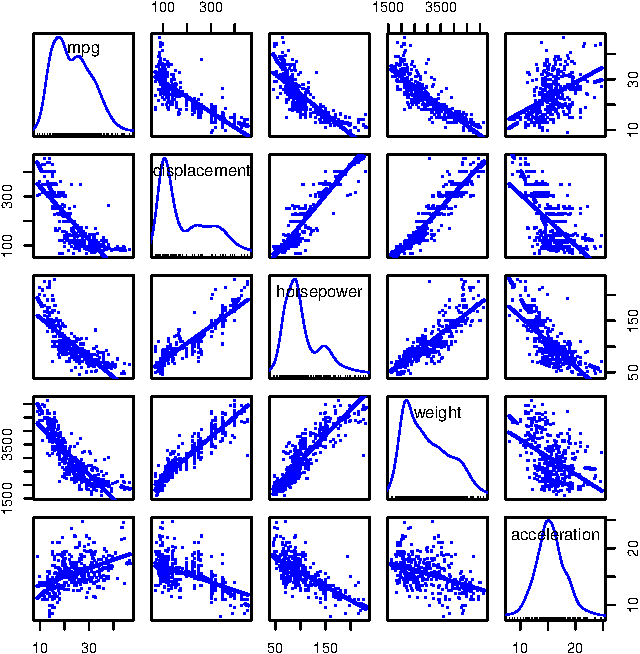
\includegraphics[width=0.6\linewidth]{JSS-article-3_files/figure-latex/Auto-explore-1} 

}

\caption[Scatterplot matrix for the numeric variables in the \code{Auto} data]{Scatterplot matrix for the numeric variables in the \code{Auto} data. In each panel, the solid line shows the linear least-squares fit and the broken line is for a nonparametric regression.}\label{fig:Auto-explore}
\end{figure}
\end{CodeChunk}

A comment before we proceed: \code{origin} is clearly categorical and so
converting it to a factor is natural, but we could imagine treating
\code{cylinders} and \code{year} as numeric predictors. There are,
however, only 5 distinct values of \code{cylinders} (ranging from 3 to
8), but cars with 3 or 5 cylinders are rare, and none of the cars has 7
cylinders. There are similarly only 13 distinct years between 1970 and
1982 in the data, and the relationship between \code{mpg} and
\code{year} is difficult to characterize.\footnote{Making the decision
  to treat \code{year} as a factor on this basis could be construed as
  cheating in the current context, which illustrates the difficulty of
  automating the whole model-selection process. It's rarely desirable,
  in our opinion, to forgo exploration of the data to ensure the purity
  of model validation. We believe, however, that it's still useful to
  automate as much of the process as we can, as illustrated here, to
  obtain a more realistic, if still biased, estimate of the predictive
  power of a model.} It's apparent that most these variables are
positively skewed and that many of the pairwise relationships among them
are nonlinear.

We start with a ``working model'' that specifies linear partial
relationships of the response to the numeric predictors:

\begin{CodeChunk}
\begin{CodeInput}
R> m.auto <- lm(mpg ~ ., data = Auto)
R> crPlots(m.auto, pch=".")
\end{CodeInput}
\begin{figure}

{\centering 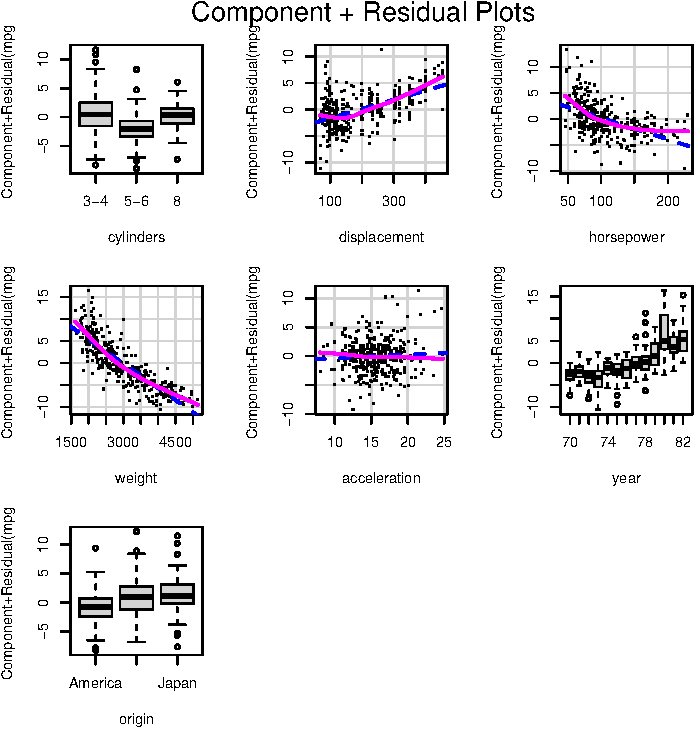
\includegraphics[width=0.6\linewidth]{JSS-article-3_files/figure-latex/Auto-working-model-1} 

}

\caption[Component+residual plots for the working model fit to the \code{Auto} data]{Component+residual plots for the working model fit to the \code{Auto} data. The broken blue lines show linear least-squares fits, while the solid magenta lines are nonparametric-regression smooths.}\label{fig:Auto-working-model}
\end{figure}
\end{CodeChunk}

The component+residual plots in Figure \ref{fig:Auto-working-model}
clearly reveal the inadequacy of the model.

Some background: As \citet[Sec. 8.2]{Weisberg:2014} explains, there are
technical advantages to having (numeric) predictors in linear regression
analysis that are themselves linearly related. If the predictors
\emph{aren't} linearly related, then the relationships between them can
often be straightened by power transformations. Transformations can be
selected after graphical examination of the data, or by analytic
methods, such as transforming the predictors towards multivariate
normality, which implies linearity. Once the relationships between the
predictors are linearized, it can be advantageous similarly to transform
the conditional distribution of the response variable towards normality.
Selecting transformations analytically raises the possibility of
automating the process, as required for cross-validation.

The \code{powerTransform()} function in the \pkg{car} package transforms
variables towards multivariate normality by a generalization of Box and
Cox's maximum-likelihood-like approach \citep{BoxCox:1964}. Several
``families'' of power transformations can be used, including the
original Box-Cox family (which is the default), simple powers (and
roots), and two adaptations of the Box-Cox family to data that may
include negative values and 0s: the Box-Cox-with-negatives family and
the Yeo-Johnson family; see \citet[Chap. 8]{Weisberg:2014} and
\citet[Chap. 3]{FoxWeisberg:2019} for details. We proceed to transform
the numeric predictors in the \code{Auto} regression towards
multivariate normality:

\begin{CodeChunk}
\begin{CodeInput}
R> num.predictors <- c("displacement", "horsepower", "weight", 
+                     "acceleration")
R> tr.x <- powerTransform(Auto[, num.predictors])
R> summary(tr.x)
\end{CodeInput}
\begin{CodeOutput}
bcPower Transformations to Multinormality 
             Est Power Rounded Pwr Wald Lwr Bnd Wald Upr Bnd
displacement   -0.0509           0      -0.2082       0.1065
horsepower     -0.1249           0      -0.2693       0.0194
weight         -0.0870           0      -0.2948       0.1208
acceleration    0.3061           0      -0.0255       0.6376

Likelihood ratio test that transformation parameters are equal to 0
 (all log transformations)
                                 LRT df    pval
LR test, lambda = (0 0 0 0) 4.872911  4 0.30059

Likelihood ratio test that no transformations are needed
                                 LRT df       pval
LR test, lambda = (1 1 1 1) 390.0777  4 < 2.22e-16
\end{CodeOutput}
\end{CodeChunk}

We then apply the (rounded) transformations---all, as it turns out, logs
(i.e., ``Oth'' powers)---to the data and re-estimate the model:

\begin{CodeChunk}
\begin{CodeInput}
R> A <- Auto
R> powers <- tr.x$roundlam
R> for (pred in num.predictors){
+   A[, pred] <- bcPower(A[, pred], lambda=powers[pred])
+ }
R> m <- update(m.auto, data=A)
\end{CodeInput}
\end{CodeChunk}

Having transformed the predictors towards multivariate normality, we now
consider whether there's evidence for transforming the response (using
\code{powerTransform()} for Box and Cox's original method), also
obtaining a log transformation:

\begin{CodeChunk}
\begin{CodeInput}
R> summary(powerTransform(m))
\end{CodeInput}
\begin{CodeOutput}
bcPower Transformation to Normality 
   Est Power Rounded Pwr Wald Lwr Bnd Wald Upr Bnd
Y1    0.0024           0      -0.1607       0.1654

Likelihood ratio test that transformation parameter is equal to 0
 (log transformation)
                               LRT df    pval
LR test, lambda = (0) 0.0008015428  1 0.97741

Likelihood ratio test that no transformation is needed
                           LRT df       pval
LR test, lambda = (1) 124.1307  1 < 2.22e-16
\end{CodeOutput}
\begin{CodeInput}
R> m <- update(m, log(mpg) ~ .)
\end{CodeInput}
\end{CodeChunk}

The transformed numeric variables are much better-behaved (cf., Figure
\ref{fig:Auto-explore}, on page \pageref{fig:Auto-explore}, and Figure
\ref{fig:Auto-transformed-scatterplot-matrix}):

\begin{CodeChunk}
\begin{CodeInput}
R> scatterplotMatrix(~ log(mpg) + displacement + horsepower + weight 
+                   + acceleration, 
+                   smooth=list(spread=FALSE), data=A, pch=".")
\end{CodeInput}
\begin{figure}

{\centering 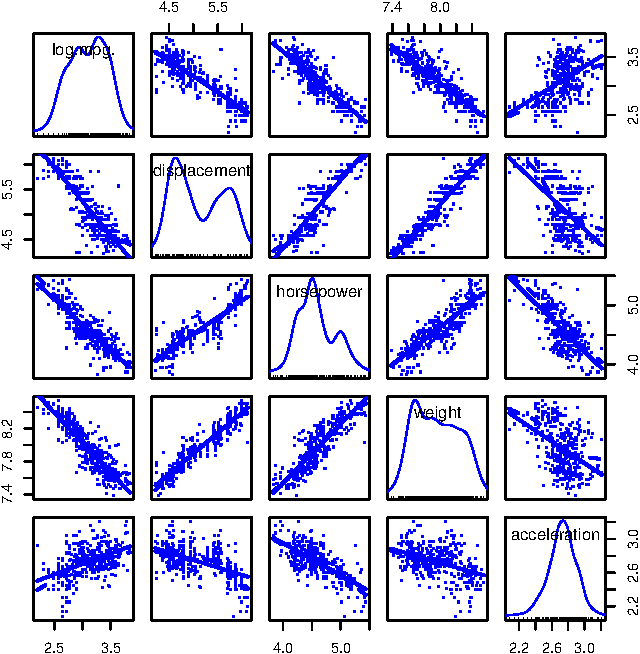
\includegraphics[width=0.6\linewidth]{JSS-article-3_files/figure-latex/Auto-transformed-scatterplot-matrix-1} 

}

\caption[Scatterplot matrix for the transformed numeric variables in the \code{Auto} data]{Scatterplot matrix for the transformed numeric variables in the \code{Auto} data}\label{fig:Auto-transformed-scatterplot-matrix}
\end{figure}
\end{CodeChunk}

And the partial relationships in the model fit to the transformed data
are much more nearly linear (cf., Figure \ref{fig:Auto-working-model},
on page \pageref{fig:Auto-working-model}, and Figure
\ref{fig:Auto-CR-plots-transformed}):

\begin{CodeChunk}
\begin{CodeInput}
R> crPlots(m, pch=".")
\end{CodeInput}
\begin{figure}

{\centering 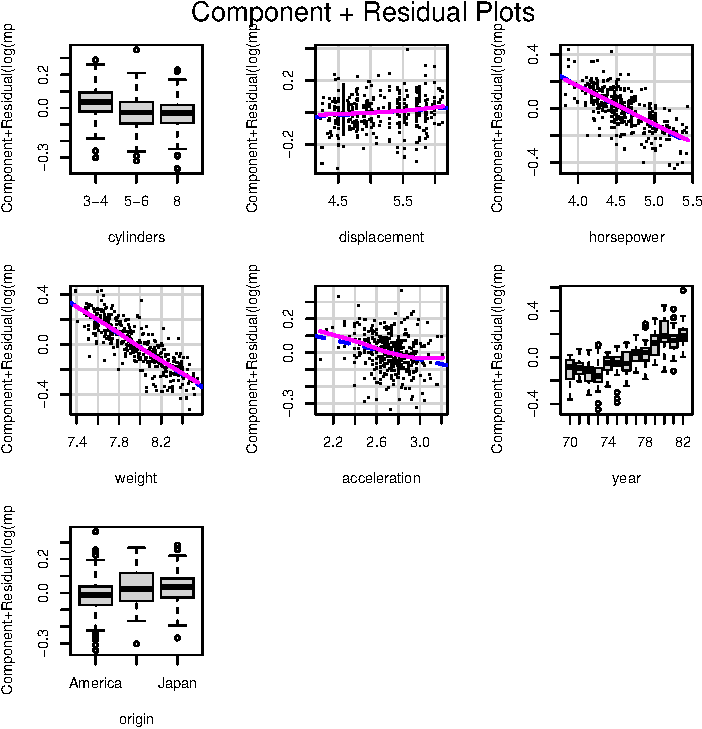
\includegraphics[width=0.6\linewidth]{JSS-article-3_files/figure-latex/Auto-CR-plots-transformed-1} 

}

\caption[Component+residual plots for the model fit to the transformed \code{Auto} data]{Component+residual plots for the model fit to the transformed \code{Auto} data}\label{fig:Auto-CR-plots-transformed}
\end{figure}
\end{CodeChunk}

After transforming both the numeric predictors and the response, we
proceed to use the \code{stepAIC()} function in the \pkg{MASS} package
to perform predictor selection, employing the BIC model-selection
criterion (by setting the \texttt{k} argument of \texttt{stepAIC()} to
\(\log n\)):

\begin{CodeChunk}
\begin{CodeInput}
R> library("MASS")
R> m.step <- stepAIC(m, k=log(nrow(A)), trace=FALSE)
R> summary(m.step)
\end{CodeInput}
\begin{CodeOutput}

Call:
lm(formula = log(mpg) ~ horsepower + weight + acceleration + 
    year + origin, data = A)

Residuals:
     Min       1Q   Median       3Q      Max 
-0.35230 -0.05682  0.00677  0.06741  0.35861 

Coefficients:
              Estimate Std. Error t value Pr(>|t|)
(Intercept)   9.434594   0.261529  36.075  < 2e-16
horsepower   -0.276254   0.056143  -4.921 1.30e-06
weight       -0.609071   0.056003 -10.876  < 2e-16
acceleration -0.131380   0.053195  -2.470  0.01397
year71        0.027984   0.028936   0.967  0.33412
year72       -0.007111   0.028446  -0.250  0.80274
year73       -0.039529   0.026014  -1.520  0.12947
year74        0.052752   0.029986   1.759  0.07936
year75        0.053199   0.029280   1.817  0.07004
year76        0.074317   0.028212   2.634  0.00878
year77        0.137931   0.028875   4.777 2.56e-06
year78        0.145876   0.027529   5.299 1.99e-07
year79        0.236036   0.029080   8.117 6.99e-15
year80        0.335274   0.031148  10.764  < 2e-16
year81        0.262872   0.030555   8.603  < 2e-16
year82        0.323391   0.029608  10.922  < 2e-16
originEurope  0.055818   0.016785   3.326  0.00097
originJapan   0.043554   0.017479   2.492  0.01314

Residual standard error: 0.1049 on 374 degrees of freedom
Multiple R-squared:  0.909, Adjusted R-squared:  0.9049 
F-statistic: 219.8 on 17 and 374 DF,  p-value: < 2.2e-16
\end{CodeOutput}
\end{CodeChunk}

The selected model includes three of the numeric predictors,
\code{horsepower}, \code{weight}, and \code{acceleration}, along with
the factors \code{year} and \code{origin}. We can calculate the MSE for
this model, but we expect that the result will be optimistic because we
used the whole data to help specify the model:

\begin{CodeChunk}
\begin{CodeInput}
R> mse(Auto$mpg, exp(fitted(m.step)))
\end{CodeInput}
\begin{CodeOutput}
[1] 6.512144
attr(,"casewise loss")
[1] "(y - yhat)^2"
\end{CodeOutput}
\end{CodeChunk}

This is considerably smaller than the MSE for the original working
model:

\begin{CodeChunk}
\begin{CodeInput}
R> mse(Auto$mpg, fitted(m.auto))
\end{CodeInput}
\begin{CodeOutput}
[1] 8.093171
attr(,"casewise loss")
[1] "(y - yhat)^2"
\end{CodeOutput}
\end{CodeChunk}

A perhaps subtle point is that we compute the MSE for the selected model
on the original \code{mpg} response scale rather than the log scale, so
as to make the selected model comparable to the working
model.\footnote{That's slightly uncomfortable given the skewed
  distribution of \code{mpg}. An alternative is to use a robust measure
  of model lack-of-fit, such as the median absolute error instead of the
  mean-squared error, employing the \code{medAbsErr()} function from the
  \pkg{cv} package. The median absolute error, however, cannot be
  expressed as a casewise average (see Section
  \ref{computation-of-the-bias-corrected-cv-criterion-and-confidence-intervals}).}

The \code{"function"} method for \code{cv()} allows us to cross-validate
the whole model-selection procedure. The first argument to
\code{cv()}---here \code{selectTransAndStepAIC}---is a model-selection
function capable of refitting the model with a fold omitted and
returning a CV criterion:

\begin{CodeChunk}
\begin{CodeInput}
R> num.predictors
\end{CodeInput}
\begin{CodeOutput}
[1] "displacement" "horsepower"   "weight"       "acceleration"
\end{CodeOutput}
\begin{CodeInput}
R> cvs <- cv(selectTransStepAIC, data=Auto, seed=76692, 
+           working.model=m.auto,
+           predictors=num.predictors,
+           response="mpg", AIC=FALSE)
\end{CodeInput}
\begin{CodeOutput}
R RNG seed set to 76692
\end{CodeOutput}
\begin{CodeInput}
R> cvs
\end{CodeInput}
\begin{CodeOutput}
10-Fold Cross Validation
criterion: mse
cross-validation criterion = 7.485557
bias-adjusted cross-validation criterion = 7.343535
full-sample criterion = 6.512144 
\end{CodeOutput}
\begin{CodeInput}
R> compareFolds(cvs)
\end{CodeInput}
\begin{CodeOutput}
CV criterion by folds:
   fold.1    fold.2    fold.3    fold.4    fold.5    fold.6    fold.7    fold.8 
 6.000589 10.509334  7.444420 10.617864  5.049238  7.183160  4.077682 10.501909 
   fold.9   fold.10 
 9.181184  4.250736 

Coefficients by folds:
        (Intercept) horsepower lam.acceleration lam.displacement lam.horsepower
Fold 1      9.71384   -0.17408          0.50000          0.00000        0.00000
Fold 2      9.21713   -0.31480          0.00000          0.00000        0.00000
Fold 3      9.61824   -0.19248          0.00000          0.00000        0.00000
Fold 4      8.69910   -0.25523          0.50000          0.00000        0.00000
Fold 5      9.14403   -0.14934          0.00000          0.00000        0.00000
Fold 6      9.63481   -0.16739          0.50000          0.00000        0.00000
Fold 7      9.98933   -0.36847          0.00000          0.00000       -0.15447
Fold 8      9.06301   -0.29721          0.00000          0.00000        0.00000
Fold 9      8.88315   -0.22684          0.00000          0.00000        0.00000
Fold 10     9.61727   -0.17086          0.00000          0.00000        0.00000
        lam.weight   lambda   weight   year71   year72   year73   year74
Fold 1     0.00000  0.00000 -0.74636  0.03764 -0.00327 -0.02477  0.05606
Fold 2     0.00000  0.00000 -0.47728  0.02173 -0.01488 -0.03770  0.04312
Fold 3     0.00000  0.00000 -0.72085  0.01128 -0.02569 -0.03872  0.05187
Fold 4     0.00000  0.00000 -0.53846  0.02153 -0.02922 -0.05181  0.04136
Fold 5     0.00000  0.00000 -0.69081  0.02531 -0.01062 -0.04625  0.05039
Fold 6     0.00000  0.00000 -0.74049  0.02456  0.00759 -0.03412  0.06266
Fold 7     0.00000  0.00000 -0.72843  0.02532 -0.01271 -0.04144  0.04568
Fold 8     0.00000  0.00000 -0.46392  0.02702 -0.02041 -0.05605  0.04437
Fold 9     0.00000  0.00000 -0.47136  0.00860 -0.03620 -0.04835  0.01906
Fold 10    0.00000  0.00000 -0.73550  0.02937 -0.00899 -0.03814  0.05408
          year75   year76   year77   year78   year79   year80   year81   year82
Fold 1   0.07080  0.07250  0.14420  0.14281  0.23266  0.35127  0.25635  0.30546
Fold 2   0.04031  0.06718  0.13094  0.14917  0.21871  0.33192  0.26196  0.30943
Fold 3   0.03837  0.06399  0.11593  0.12601  0.20499  0.32821  0.24478  0.29204
Fold 4   0.04072  0.05537  0.12292  0.14083  0.22878  0.32947  0.25140  0.27248
Fold 5   0.05596  0.07044  0.13356  0.14724  0.24675  0.33331  0.26938  0.32594
Fold 6   0.06940  0.07769  0.14211  0.14647  0.23532  0.34761  0.26737  0.33062
Fold 7   0.03614  0.07385  0.12976  0.14040  0.23976  0.33998  0.27652  0.30659
Fold 8   0.06573  0.08135  0.13158  0.13987  0.23011  0.32880  0.25886  0.30538
Fold 9   0.03018  0.05846  0.10536  0.11722  0.20665  0.31533  0.23352  0.29375
Fold 10  0.04881  0.07862  0.14101  0.14313  0.23258  0.35649  0.26214  0.32421
        acceleration displacement cylinders5-6 cylinders8 originEurope
Fold 1                                                                
Fold 2      -0.18909     -0.09197                                     
Fold 3                                                                
Fold 4      -0.03484                  -0.09080   -0.10909             
Fold 5                                                         0.06261
Fold 6                                                                
Fold 7                                                                
Fold 8      -0.17676     -0.10542                                     
Fold 9      -0.14514     -0.13452                                     
Fold 10                                                               
        originJapan
Fold 1             
Fold 2             
Fold 3             
Fold 4             
Fold 5         0.04
Fold 6             
Fold 7             
Fold 8             
Fold 9             
Fold 10            
\end{CodeOutput}
\end{CodeChunk}

The other arguments to \code{cv()} are (see \code{?cv:::cv.function} for
additional optional arguments and details):

\begin{itemize}
\tightlist
\item
  \code{data}, the data set to which the model is fit.
\item
  \code{seed}, an optional seed for \proglang{R}'s pseudo-random-number
  generator; as for \code{cv()}, if the seed isn't supplied by the user,
  then a seed is randomly selected and saved.
\item
  Arguments required by the model-selection function: the starting
  \code{working.model} (here, \code{m.auto}) for transformation and
  predictor selection; the names of the variables---\code{predictors}
  and \code{response}---that are candidates for transformation; and
  \code{AIC=FALSE}, which specifies use of the BIC for model selection.
\end{itemize}

Some noteworthy points:

\begin{itemize}
\tightlist
\item
  \code{selectTransStepAIC()} automatically computes CV cost criteria,
  here the MSE, on the \emph{untransformed} response scale.
\item
  As we anticipated, the estimate of the MSE that we obtain by
  cross-validating the whole model-specification process is larger than
  the MSE computed for the model we fit to the \code{Auto} data
  separately selecting transformations of the predictors and the
  response and then selecting predictors for the whole data set.
\item
  When we look at the transformations and predictors selected with each
  of the 10 folds omitted (i.e., the output of \code{compareFolds()}),
  we see that there is little uncertainty in choosing variable
  transformations (the \code{lam.*}s for the \(x\)s and \code{lambda}
  for \(y\) in the output), but considerably more uncertainty in
  subsequently selecting predictors: \code{horsepower}, \code{weight},
  and \code{year} are always included among the selected predictors;
  \code{acceleration} and \code{displacement} are included respectively
  in 4 and 3 of 10 selected models; and \code{cylinders} and
  \code{origin} are each included in only 1 of 10 models. Recall that
  when we selected predictors for the full data, we obtained a model
  with \code{horsepower}, \code{weight}, \code{acceleration},
  \code{year}, and \code{origin}.
\end{itemize}

\subsection{Example: Applying recursive CV to polynomial regression for
the Auto
data}\label{example-applying-recursive-cv-to-polynomial-regression-for-the-auto-data}

In Section \ref{comparing-competing-models}, following \citet[Secs. 5.1,
5.3]{JamesEtAl:2021}, we fit polynomial regressions up to degree 10 to
the relationship of \texttt{mpg} to \texttt{horsepower} for the
\texttt{Auto} data, saving the 10 models, named \texttt{m.1} through
\texttt{m.10}, in \texttt{mlist}. We then used \texttt{cv()} to compare
the cross-validated MSE for the 10 models, discovering that the 7th
degree polynomial had the smallest MSE (by a small margin).

If we then select the 7th degree polynomial model, intending to use it
for prediction, the CV estimate of the MSE for this model will be
optimistic. One solution is to cross-validate the process of using CV to
select the ``best'' model---that is, to apply CV to CV recursively. The
function \texttt{selectModelList()}, which is suitable for use with
\texttt{cv()}, implements this idea.

Applying \texttt{selectModelList()} to the \texttt{Auto}
polynomial-regression models, and using 10-fold CV, we obtain:

\begin{CodeChunk}
\begin{CodeInput}
R> recursiveCV.auto <- cv(selectModelList, data=Auto, 
+                        working.model=mlist,
+                        save.model=TRUE, seed=2120)
\end{CodeInput}
\begin{CodeOutput}
R RNG seed set to 2120
\end{CodeOutput}
\begin{CodeInput}
R> recursiveCV.auto
\end{CodeInput}
\begin{CodeOutput}
10-Fold Cross Validation
criterion: mse
cross-validation criterion = 20.01249
bias-adjusted cross-validation criterion = 20.61866
full-sample criterion = 18.74615 
\end{CodeOutput}
\begin{CodeInput}
R> recursiveCV.auto$selected.model
\end{CodeInput}
\begin{CodeOutput}

Call:
lm(formula = mpg ~ poly(horsepower, p), data = Auto)

Coefficients:
         (Intercept)  poly(horsepower, p)1  poly(horsepower, p)2  
              23.446              -120.138                44.090  
poly(horsepower, p)3  poly(horsepower, p)4  poly(horsepower, p)5  
              -3.949                -5.188                13.272  
poly(horsepower, p)6  poly(horsepower, p)7  
              -8.546                 7.981  
\end{CodeOutput}
\begin{CodeInput}
R> cv(mlist[[7]], seed=2120) # same seed for same folds
\end{CodeInput}
\begin{CodeOutput}
R RNG seed set to 2120
\end{CodeOutput}
\begin{CodeOutput}
10-Fold Cross Validation
method: Woodbury
criterion: mse
cross-validation criterion = 18.89822
bias-adjusted cross-validation criterion = 18.85429
full-sample criterion = 18.07817 
\end{CodeOutput}
\end{CodeChunk}

As expected, recursive CV produces a larger estimate of MSE for the
selected 7th degree polynomial model than CV applied directly to this
model.

We can equivalently call \texttt{cv()} with the list of models as its
first argument and set the argument \texttt{recursive=TRUE}:

\begin{CodeChunk}
\begin{CodeInput}
R> cv(mlist, data=Auto, seed=2120, recursive=TRUE, save.model=TRUE)
\end{CodeInput}
\begin{CodeOutput}
R RNG seed set to 2120
\end{CodeOutput}
\begin{CodeOutput}
10-Fold Cross Validation
cross-validation criterion = 20.01249
bias-adjusted cross-validation criterion = 20.61866
full-sample criterion = 18.74615 
\end{CodeOutput}
\end{CodeChunk}

\section{Extending the cv package}\label{extending-the-cv-package}

The \pkg{cv} package is designed to be extensible in several directions.
In order of increasing general complexity, we can add: (1) a
cross-validation cost criterion; (2) a model class that's not directly
accommodated by the \code{cv()} default method or by another directly
inherited method; and (3) a new model-selection procedure suitable for
use with the \code{"function"} method for \code{cv()}. In this section,
we illustrate (1) and (2); more diverse and extensive examples may be
found in the vignette on extending the \pkg{cv} package.

Suppose that we want to cross-validate a multinomial logistic regression
model fit by the \code{multinom()} function in the \pkg{nnet} package
\citep{VenablesRipley:2002}. We borrow an example from \citet[Sec.
14.2.1]{Fox:2016}, with data from the British Election Panel Study on
vote choice in the 2001 British election. Data for the example are in
the \code{BEPS} data set in the \pkg{carData} package:

\begin{CodeChunk}
\begin{CodeInput}
R> data("BEPS", package="carData")
R> summary(BEPS)
\end{CodeInput}
\begin{CodeOutput}
               vote          age        economic.cond.national
 Conservative    :462   Min.   :24.00   Min.   :1.000         
 Labour          :720   1st Qu.:41.00   1st Qu.:3.000         
 Liberal Democrat:343   Median :53.00   Median :3.000         
                        Mean   :54.18   Mean   :3.246         
                        3rd Qu.:67.00   3rd Qu.:4.000         
                        Max.   :93.00   Max.   :5.000         
 economic.cond.household     Blair           Hague          Kennedy     
 Min.   :1.00            Min.   :1.000   Min.   :1.000   Min.   :1.000  
 1st Qu.:3.00            1st Qu.:2.000   1st Qu.:2.000   1st Qu.:2.000  
 Median :3.00            Median :4.000   Median :2.000   Median :3.000  
 Mean   :3.14            Mean   :3.334   Mean   :2.747   Mean   :3.135  
 3rd Qu.:4.00            3rd Qu.:4.000   3rd Qu.:4.000   3rd Qu.:4.000  
 Max.   :5.00            Max.   :5.000   Max.   :5.000   Max.   :5.000  
     Europe       political.knowledge    gender   
 Min.   : 1.000   Min.   :0.000       female:812  
 1st Qu.: 4.000   1st Qu.:0.000       male  :713  
 Median : 6.000   Median :2.000                   
 Mean   : 6.729   Mean   :1.542                   
 3rd Qu.:10.000   3rd Qu.:2.000                   
 Max.   :11.000   Max.   :3.000                   
\end{CodeOutput}
\end{CodeChunk}

The polytomous (multi-category) response variable is \code{vote}, a
factor with levels \code{"Conservative"}, \code{"Labour"}, and
\code{"Liberal Democrat"}. The predictors of \code{vote} are:

\begin{itemize}
\tightlist
\item
  \code{age}, in years;
\item
  \code{econ.cond.national} and \code{econ.cond.household}, the
  respondent's ratings of the state of the economy, on 1 to 5 scales.
\item
  \code{Blair}, \code{Hague}, and \code{Kennedy}, ratings of the leaders
  of the Labour, Conservative, and Liberal Democratic parties, on 1 to 5
  scales.
\item
  \code{Europe}, an 11-point scale on attitude towards European
  integration, with high scores representing ``Euro-skepticism.''
\item
  \code{political.knowledge}, knowledge of the parties' positions on
  European integration, with scores from 0 to 3.
\item
  \code{gender}, \code{"female"} or \code{"male"}.
\end{itemize}

The model fit to the data includes an interaction between \code{Europe}
and \code{political.knowledge}, which was the focus of the original
research on which this example is based
\citep{AndersenHeathSinnott:2002}; the other predictors enter the model
additively:

\begin{CodeChunk}
\begin{CodeInput}
R> library("nnet", quietly=TRUE)
R> m.beps <- multinom(vote ~ age + gender + economic.cond.national +
+                        economic.cond.household + Blair + Hague + Kennedy +
+                        Europe*political.knowledge, data=BEPS)
\end{CodeInput}
\begin{CodeOutput}
# weights:  36 (22 variable)
initial  value 1675.383740 
iter  10 value 1240.047788
iter  20 value 1163.199642
iter  30 value 1116.519687
final  value 1116.519666 
converged
\end{CodeOutput}
\end{CodeChunk}

The \code{Europe} \(\times\) \code{political.knowledge} interaction is
associated with a very small \(p\)-value. Figure \ref{fig:BEPS-plot}
shows an ``effect plot,'' using the the \pkg{effects} package
\citep{FoxWeisberg:2019} to visualize the interaction in a
``stacked-area'' graph:

\begin{CodeChunk}
\begin{CodeInput}
R> plot(effects::Effect(c("Europe", "political.knowledge"), m.beps,
+             xlevels=list(Europe=1:11, political.knowledge=0:3),
+             fixed.predictors=list(given.values=c(gendermale=0.5))),
+      lines=list(col=c("blue", "red", "orange")), # party colors
+      axes=list(x=list(rug=FALSE), y=list(style="stacked")))
\end{CodeInput}
\begin{figure}

{\centering 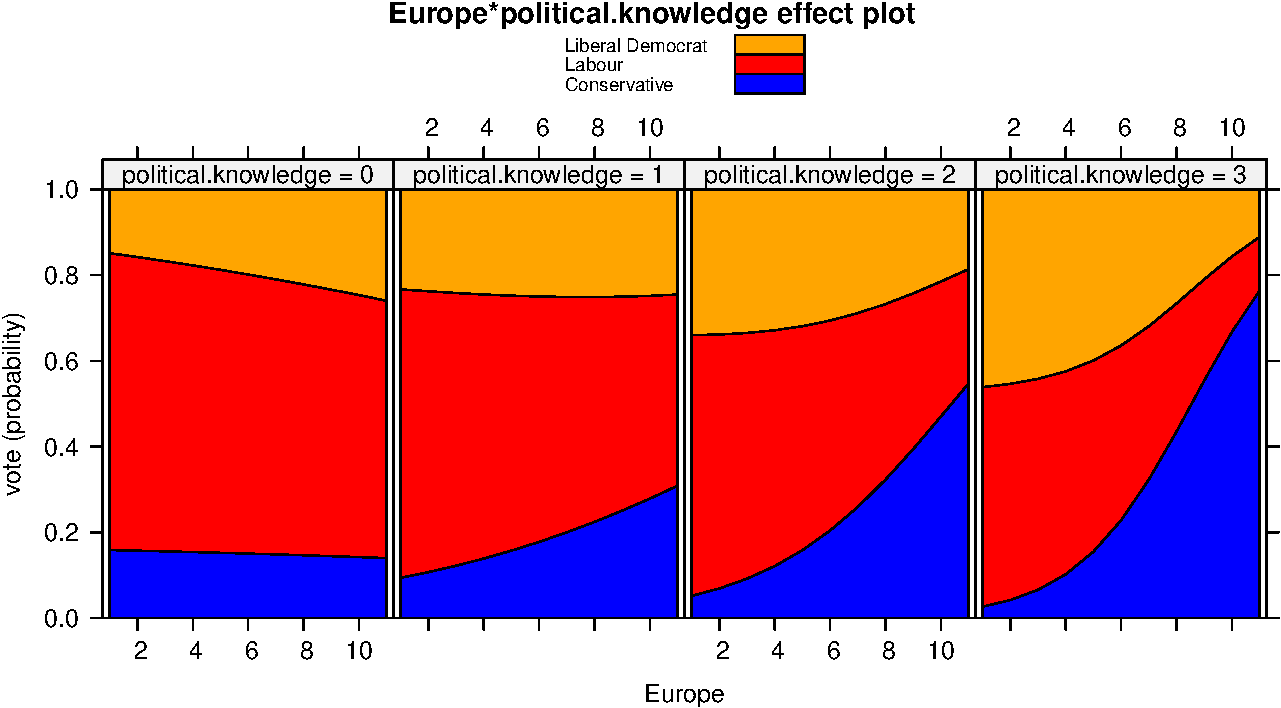
\includegraphics{JSS-article-3_files/figure-latex/BEPS-plot-1} 

}

\caption[Effect plot for the interaction between attitude towards European integration and political knowledge in the multinomial logit model fit to voting data from the 2001 British Election Panel Study]{Effect plot for the interaction between attitude towards European integration and political knowledge in the multinomial logit model fit to voting data from the 2001 British Election Panel Study.}\label{fig:BEPS-plot}
\end{figure}
\end{CodeChunk}

As political knowledge increases, voters tend to align their votes more
closely with the party positions on European integration: The
Conservative Party was relatively Euro-skeptic, while Labour and the
Liberal Democrats were more supportive of the UK's participation in the
EU.

To cross-validate this multinomial-logit model we need an appropriate
cost criterion. None of the criteria in the \pkg{cv} package will
do---for example, \code{mse()} is appropriate only for a numeric
response. The \code{BayesRule()} criterion, also supplied by \pkg{cv},
which is for a binary response, comes close:

\begin{CodeChunk}
\begin{CodeInput}
R> BayesRule
\end{CodeInput}
\begin{CodeOutput}
function(y, yhat) {
  if (!all(y %in% c(0, 1)))
    stop("response values not all 0 or 1")
  if (any(yhat < 0) ||
      any(yhat > 1))
    stop("fitted values outside of interval [0, 1]")
  yhat <- round(yhat)
  result <- mean(y != yhat) # proportion in error
  attr(result, "casewise loss") <- "y != round(yhat)"
  result
}
<bytecode: 0x14013a7f0>
<environment: namespace:cv>
\end{CodeOutput}
\end{CodeChunk}

After doing some error checking, \code{BayesRule()} rounds the predicted
proabability of a 1 (``success'') response in a binary regression model
to 0 or 1 to obtain a categorical prediction, and then reports the
proportion of incorrect predictions. Because the Bayes's rule criterion
is an average of casewise components (as, e.g., is the MSE), a
\code{"casewise loss"} attribute is attached to the result, enabling the
computation of bias correction and confidence intervals (as discussed in
Section
\ref{computation-of-the-bias-corrected-cv-criterion-and-confidence-intervals}).

It is straightforward to adapt Bayes's rule to a polytomous response:

\begin{CodeChunk}
\begin{CodeInput}
R> head(BEPS$vote)
\end{CodeInput}
\begin{CodeOutput}
[1] Liberal Democrat Labour           Labour           Labour          
[5] Labour           Labour          
Levels: Conservative Labour Liberal Democrat
\end{CodeOutput}
\begin{CodeInput}
R> yhat <- predict(m.beps, type="class")
R> head(yhat)
\end{CodeInput}
\begin{CodeOutput}
[1] Labour           Labour           Labour           Labour          
[5] Liberal Democrat Labour          
Levels: Conservative Labour Liberal Democrat
\end{CodeOutput}
\begin{CodeInput}
R> BayesRuleMulti <- function(y, yhat){
+   result <- mean(y != yhat)
+   attr(result, "casewise loss") <- "y != yhat"
+   result
+ }
R> 
R> BayesRuleMulti(BEPS$vote, yhat)
\end{CodeInput}
\begin{CodeOutput}
[1] 0.3186885
attr(,"casewise loss")
[1] "y != yhat"
\end{CodeOutput}
\end{CodeChunk}

The \code{predict()} method for \code{"multinom"} models called with
argument \code{type="class"} reports the Bayes's rule prediction for
each case---that is, the response category with the highest predicted
probability. Our \code{BayesRuleMulti()} function calculates the
proportion of misclassified cases. Because this value is also the mean
of casewise components, we attach a \code{"casewise loss"} attribute to
the result.

The marginal proportions for the response categories are

\begin{CodeChunk}
\begin{CodeInput}
R> xtabs(~ vote, data=BEPS)/nrow(BEPS)
\end{CodeInput}
\begin{CodeOutput}
vote
    Conservative           Labour Liberal Democrat 
       0.3029508        0.4721311        0.2249180 
\end{CodeOutput}
\end{CodeChunk}

and so the marginal Bayes's rule prediction, that everyone will vote
Labour, produces an error rate of \(1 - 0.47213 = 0.52787\). The
multinomial-logit model appears to do substantially better than that,
but does its performance hold up to cross-validation?

We check first whether the default \code{cv()} method works
``out-of-the-box'' for the \code{"multinom"} model:

\begin{CodeChunk}
\begin{CodeInput}
R> cv(m.beps, seed=3465, criterion=BayesRuleMulti)
\end{CodeInput}
\begin{CodeOutput}
Error in GetResponse.default(model): non-vector response
\end{CodeOutput}
\end{CodeChunk}

The default method of \code{GetResponse()} (a function supplied by the
\pkg{cv} package---see \code{?GetResponse}) fails for a
\code{"multinom"} object. A straightforward solution is to supply a
\code{GetResponse.multinom()} method that returns the factor response
\citep[using the \texttt{get\_response()} function from the
\pkg{insight} package,][]{LudeckeWaggonerMakowski:2019},

\begin{CodeChunk}
\begin{CodeInput}
R> GetResponse.multinom <- function(model, ...) {
+   insight::get_response(model)
+ }
R> 
R> head(GetResponse(m.beps))
\end{CodeInput}
\begin{CodeOutput}
[1] Liberal Democrat Labour           Labour           Labour          
[5] Labour           Labour          
Levels: Conservative Labour Liberal Democrat
\end{CodeOutput}
\end{CodeChunk}

and to try again:

\begin{CodeChunk}
\begin{CodeInput}
R> cv(m.beps, seed=3465, criterion=BayesRuleMulti)
\end{CodeInput}
\begin{CodeOutput}
R RNG seed set to 3465
\end{CodeOutput}
\begin{CodeOutput}
# weights:  36 (22 variable)
initial  value 1507.296060 
iter  10 value 1134.575036
iter  20 value 1037.413231
iter  30 value 1007.705242
iter  30 value 1007.705235
iter  30 value 1007.705235
final  value 1007.705235 
converged
\end{CodeOutput}
\begin{CodeOutput}
Error in match.arg(type): 'arg' should be one of "class", "probs"
\end{CodeOutput}
\end{CodeChunk}

A \code{traceback()} (not shown) reveals that the problem is that the
default method of \code{cv()} calls the \code{"multinom"} method for
\code{predict()} with the argument \code{type="response"}, when the
correct argument should be \code{type="class"}. We therefore must write
a \code{"multinom"} method for \code{cv()}, but that proves to be very
simple:

\begin{CodeChunk}
\begin{CodeInput}
R> cv.multinom <- function (model, data, criterion = BayesRuleMulti, 
+                          k, reps, seed, ...) {
+     model <- update(model, trace = FALSE)
+     NextMethod(
+       type = "class",
+       criterion = criterion,
+       criterion.name = deparse(substitute(criterion))
+     )
+   }
\end{CodeInput}
\end{CodeChunk}

That is, we simply call the default \texttt{cv()} method (via
\code{NextMethod()}) with the \texttt{type} argument properly set. In
addition to supplying the correct \texttt{type} argument, our method
sets the default \texttt{criterion} for the \texttt{cv.multinom()}
method to \texttt{BayesRuleMulti}. Adding the argument
\texttt{criterion.name=} \texttt{deparse(substitute(criterion))} is
inessential, but it insures that printed output will include the name of
the criterion function that's employed, whether it's the default
\texttt{BayesRuleMulti} or something else. Prior to invoking
\texttt{NextMethod()}, we called \texttt{update()} with
\texttt{trace=FALSE} to suppress the iteration history reported by
default by \texttt{multinom()}---it would be tedious to see the
iteration history for each fold.

Then:

\begin{CodeChunk}
\begin{CodeInput}
R> cv(m.beps, seed=3465)
\end{CodeInput}
\begin{CodeOutput}
R RNG seed set to 3465
\end{CodeOutput}
\begin{CodeOutput}
10-Fold Cross Validation
criterion: BayesRuleMulti
cross-validation criterion = 0.3245902
bias-adjusted cross-validation criterion = 0.3236756
95% CI for bias-adjusted CV criterion = (0.300168, 0.3471831)
full-sample criterion = 0.3186885 
\end{CodeOutput}
\end{CodeChunk}

The cross-validated polytomous Bayes's rule criterion confirms that the
fitted model does substantially better than the marginal Bayes's rule
prediction that everyone votes for Labour.

\section{Comparing cv to other R software for
cross-validation}\label{comparing-cv-to-other-r-software-for-cross-validation}

The \pkg{cv} package is far from unique in implementing cross-validation
of regression models in \proglang{R}. We've already mentioned the
\code{cv.glm()} function in the \pkg{boot} package. A general review of
CV facilities in \proglang{R} is beyond the scope of the current paper,
but in this section we remark selectively on other \proglang{R} packages
that support CV.

Our goal in implementing CV is to make it conveniently available to
\proglang{R} users with limited programming skills,\footnote{\proglang{R}
  users with sophisticated programming skills would generally find it
  unchallenging to implement CV directly for specific applications. Even
  in this case, however, there's an argument for using a simple
  pre-programmed interface to CV, to minimize programming effort and to
  avoid mistakes.} and hence to encourage its use. Towards this end, the
\pkg{cv} package provides a simple, consistent interface through the
\code{cv()} generic function, with specific methods for different
classes of standard \proglang{R} statistical models. Moreover, we have
tried to make writing methods for additional classes of statistical
models as simple and straightforward as possible. Because CV is
computationally intensive, we also aim for efficiency, by enabling
parallel computations generally, and by exploiting properties of
specific classes of statistical models (in particular, computations
based on hatvalues and the Woodbury matrix identity for linear and
generalized linear model). Finally, the package includes some unusual
features, such as general support for mixed-effects models and for
cross-validating complex model-specification procedures.

Some \proglang{R} packages for statistical learning include facilities
for cross-validation. Notable examples are the \pkg{caret} package
\citep{Kuhn:2008} and the \pkg{tidyfit} package \citep{Pfitzinger:2024};
the latter employs \pkg{rsample} \citep{FrickEtAl:2024} for CV, which we
will discuss presently This contrasts with the approach taken in the
\pkg{cv} package, which, as we have explained, directly supports classes
of standard \proglang{R} statistical models.

Other packages, including \pkg{cvms} \citep{OlsenZachariae:2024},
\pkg{mlexperiments} \citep{Kapsner:2024}, \pkg{origami}
\citep{CoyleEtAl:2022}, and \pkg{rsample} (which also supports
bootstrapping), modularize the CV process to a greater or lesser extent.
Advantages of this approach include flexibility and generality, but a
disadvantage is that use of these packages entails nontrivial
programming effort and skill.

We illustrate with an example adapted from a vignette in the
\pkg{rsample} package, which uses the \code{attrition} data set from the
\pkg{modeldata} package. Here, with minimal explanation, is how one
would perform LOO CV for the example using \pkg{rsample}:\footnote{The
  example in the \pkg{rsample} vignette uses 10-fold rather than LOO CV,
  but otherwise the code from the vignette is only trivially modified
  here.}

\begin{CodeChunk}
\begin{CodeInput}
R> library(rsample)
R> 
R> data("attrition", package = "modeldata")
R> nrow(attrition)
\end{CodeInput}
\begin{CodeOutput}
[1] 1470
\end{CodeOutput}
\begin{CodeInput}
R> # formula for model to be fit; Attrition is binary:
R> mod_form <- Attrition ~ JobSatisfaction + Gender + MonthlyIncome
R> 
R> rs_obj <- loo_cv(attrition) # original uses vfold_cv()
R> 
R> # user-supplied function:
R> holdout_results <- function(splits, ...) {
+   mod <- glm(..., data=analysis(splits), family=binomial)
+   holdout <- assessment(splits)
+   res <- broom::augment(mod, newdata=holdout)
+   lvls <- levels(holdout$Attrition)
+   predictions <- factor(ifelse(res$.fitted > 0, lvls[2], lvls[1]),
+                         levels=lvls)
+   res$correct <- predictions == holdout$Attrition
+   res
+ }
R> 
R> library(purrr, quietly=TRUE)
R> # apply CV:
R> rs_obj$results <- map(rs_obj$splits, holdout_results, mod_form)
R> # summarize results:
R> rs_obj$accuracy <- map_dbl(rs_obj$results,
+                            function(x) mean(x$correct))
R> # accuracy is the complement of the Bayes-rule CV criterion:
R> 1 - summary(rs_obj$accuracy) 
\end{CodeInput}
\begin{CodeOutput}
   Min. 1st Qu.  Median    Mean 3rd Qu.    Max. 
 1.0000  0.0000  0.0000  0.1612  0.0000  0.0000 
\end{CodeOutput}
\end{CodeChunk}

And here's how we can perform the same computation using the \code{cv()}
function in the \pkg{cv} package:

\begin{CodeChunk}
\begin{CodeInput}
R> mod.attrition <- glm(mod_form, data=attrition, family=binomial)
R> (cv.attrition <- cv(mod.attrition, k="loo", criterion=BayesRule))
\end{CodeInput}
\begin{CodeOutput}
n-Fold Cross Validation
method: exact
criterion: BayesRule
cross-validation criterion = 0.1612245
bias-adjusted cross-validation criterion = 0.1612245
95% CI for bias-adjusted CV criterion = (0.1424194, 0.1800296)
full-sample criterion = 0.1612245 
\end{CodeOutput}
\end{CodeChunk}

Let's compare the computational efficiency of the two implementations,
also showing the use of \code{method="Woodbury"} and
\code{method="hatvalues"} for \code{cv()}, which, in this example,
produce numerically identical results to the default
\code{method="exact"}:

\begin{CodeChunk}
\begin{CodeInput}
R> all.equal(cv.attrition$`CV crit`,
+           cv(mod.attrition, k="loo", criterion=BayesRule,
+              method="Woodbury")$`CV crit`,
+           )
\end{CodeInput}
\begin{CodeOutput}
[1] TRUE
\end{CodeOutput}
\begin{CodeInput}
R> all.equal(cv.attrition$`CV crit`,
+           cv(mod.attrition, k="loo", criterion=BayesRule,
+              method="hatvalues")$`CV crit`
+           )
\end{CodeInput}
\begin{CodeOutput}
[1] TRUE
\end{CodeOutput}
\begin{CodeInput}
R> microbenchmark::microbenchmark(
+   rsample={
+     rs_obj$results <- map(rs_obj$splits, holdout_results, mod_form)
+     rs_obj$accuracy <- map_dbl(rs_obj$results,
+                                function(x) mean(x$correct))
+   },
+   cv.exact=cv(mod.attrition, k="loo", criterion=BayesRule),
+   cv.wood=cv(mod.attrition, k="loo", criterion=BayesRule,
+              method="Woodbury"),
+   cv.hatvalues=cv(mod.attrition, k="loo", criterion=BayesRule,
+                   method="hatvalues"),
+   times=10
+ )
\end{CodeInput}
\begin{CodeOutput}
Warning in microbenchmark::microbenchmark(rsample = {: less accurate nanosecond
times to avoid potential integer overflows
\end{CodeOutput}
\begin{CodeOutput}
Unit: milliseconds
         expr         min          lq        mean      median          uq
      rsample 5814.989369 5864.285227 5952.773502 5897.248509 6023.438043
     cv.exact 4739.827837 4827.064193 4902.546681 4910.249278 4952.683150
      cv.wood  103.663047  104.760125  110.628578  111.201532  116.027007
 cv.hatvalues    1.217905    1.222251    1.409719    1.479649    1.543937
         max neval
 6207.205988    10
 5090.904318    10
  118.610540    10
    1.591538    10
\end{CodeOutput}
\end{CodeChunk}

Computing time for \pkg{rsample} for this problem is similar to
\code{cv()} with \code{method="exact"}, but more than an order of
magitude slower than \code{cv()} with \code{method="Woodbury"}, and more
than three orders of magnitude slower then \code{cv()} with
\code{method="hatvalues"}.

\section{Computational notes}\label{computational-notes}

\subsection{Efficient computations for linear and generalized linear
models}\label{efficient-computations-for-linear-and-generalized-linear-models}

The most straightforward way to implement cross-validation in
\proglang{R} for statistical modeling functions that are written in the
canonical manner is to use \code{update()} to refit the model with each
fold removed. This is the approach taken in the default method for
\code{cv()}, and it is appropriate if the cases are independently
sampled. Refitting the model in this manner for each fold is generally
feasible when the number of folds in modest, but can be prohibitively
costly for leave-one-out cross-validation when the number of cases is
large.

The \code{"lm"} and \code{"glm"} methods for \code{cv()} take advantage
of computational efficiencies by avoiding refitting the model with each
fold removed. Consider, in particular, the weighted linear model
\(\mathbf{y}_{n \times 1} = \mathbf{X}_{n \times p}\boldsymbol{\beta}_{p \times 1} + \boldsymbol{\varepsilon}_{n \times 1}\),
where
\(\boldsymbol{\varepsilon} \sim \mathbf{N}_n \left(\mathbf{0}, \sigma^2 \mathbf{W}^{-1}_{n \times n}\right)\).
Here, \(\mathbf{y}\) is the response vector, \(\mathbf{X}\) the model
matrix, and \(\boldsymbol{\varepsilon}\) the error vector, each for
\(n\) cases, and \(\boldsymbol{\beta}\) is the vector of \(p\)
population regression coefficients. The errors are assumed to be
multivariately normally distributed with 0 means and covariance matrix
\(\sigma^2 \mathbf{W}^{-1}\), where \(\mathbf{W} = \mathrm{diag}(w_i)\)
is a diagonal matrix of inverse-variance weights. For the linear model
with constant error variance, the weight matrix is taken to be
\(\mathbf{W} = \mathbf{I}_n\), the order-\(n\) identity matrix.

The weighted-least-squares (WLS) estimator of \(\boldsymbol{\beta}\) is
\citep[see, e.g.,][Sec. 12.2.2]{Fox:2016} \footnote{This is a
  definitional formula, which assumes that the model matrix
  \(\mathbf{X}\) is of full column rank, and which can be subject to
  numerical instability when \(\mathbf{X}\) is ill-conditioned.
  \code{lm()} uses the singular-value decomposition of the model matrix
  to obtain computationally more stable results.} \[
\mathbf{b}_{\mathrm{WLS}} = \left( \mathbf{X}^T \mathbf{W} \mathbf{X} \right)^{-1} 
  \mathbf{X}^T \mathbf{W} \mathbf{y}
\]

Fitted values are then
\(\widehat{\mathbf{y}} = \mathbf{X}\mathbf{b}_{\mathrm{WLS}}\).

The LOO fitted value for the \(i\)th case can be efficiently computed by
\(\widehat{y}_{-i} = y_i - e_i/(1 - h_i)\) where
\(h_i = \mathbf{x}^T_i \left( \mathbf{X}^T \mathbf{W} \mathbf{X} \right)^{-1} \mathbf{x}_i\)
(the so-called ``hatvalue''). Here, \(\mathbf{x}^T_i\) is the \(i\)th
row of \(\mathbf{X}\), and \(\mathbf{x}_i\) is the \(i\)th row written
as a column vector. This approach can break down when one or more
hatvalues are equal to 1, in which case the formula for
\(\widehat{y}_{-i}\) requires division by 0. In this case, the
``training'' set omitting the observation with hatvalue = 1 is
rank-deficient and the predictors for the left-out case are outside the
linear span of the predictors in the training set.

To compute cross-validated fitted values when the folds contain more
than one case, we make use of the Woodbury matrix identify
\citep{Hager:1989}, \[
\left(\mathbf{A}_{m \times m} + \mathbf{U}_{m \times k} 
\mathbf{C}_{k \times k} \mathbf{V}_{k \times m} \right)^{-1} = \mathbf{A}^{-1} - \mathbf{A}^{-1}\mathbf{U} \left(\mathbf{C}^{-1} + 
\mathbf{VA}^{-1}\mathbf{U} \right)^{-1} \mathbf{VA}^{-1}
\] where \(\mathbf{A}\) is a nonsingular order-\(n\) matrix. We apply
this result by letting \begin{align*}
    \mathbf{A} &= \mathbf{X}^T \mathbf{W} \mathbf{X} \\
    \mathbf{U} &= \mathbf{X}_\mathbf{j}^T \\
    \mathbf{V} &= - \mathbf{X}_\mathbf{j} \\
    \mathbf{C} &= \mathbf{W}_\mathbf{j} \\
\end{align*} where the subscript
\(\mathbf{j} = (i_{j1}, \ldots, i_{jm})^T\) represents the vector of
indices for the cases in the \(j\)th fold, \(j = 1, \ldots, k\). The
negative sign in \(\mathbf{V} = - \mathbf{X}_\mathbf{j}\) reflects the
\emph{removal}, rather than addition, of the cases in \(\mathbf{j}\).

Applying the Woodbury identity isn't quite as fast as using the
hatvalues, but it is generally much faster than refitting the model. A
disadvantage of the Woodbury identity, however, is that it entails
explicit matrix inversion and thus may be numerically unstable. The
inverse of \(\mathbf{A} = \mathbf{X}^T \mathbf{W} \mathbf{X}\) is
available directly in the \code{"lm"} object, but the second term on the
right-hand side of the Woodbury identity requires a matrix inversion
with each fold deleted. (In contrast, the inverse of each
\(\mathbf{C} = \mathbf{W}_\mathbf{j}\) is straightforward because
\(\mathbf{W}\) is diagonal.)

The Woodbury identity also requires that the model matrix be of full
rank. We impose that restriction in our code by removing redundant
regressors from the model matrix for all of the cases, but that doesn't
preclude rank deficiency from surfacing when a fold is removed. Rank
deficiency of \(\mathbf{X}\) doesn't disqualify cross-validation because
all we need are fitted values under the estimated model.

\code{glm()} computes the maximum-likelihood estimates for a generalized
linear model by iterated weighted least squares \citep[see, e.g.,][Sec.
6.12]{FoxWeisberg:2019}. The last iteration is therefore just a WLS fit
of the ``working response'' on the model matrix using ``working
weights.'' Both the working weights and the working response at
convergence are available from the information in the object returned by
\code{glm()}.

We then treat re-estimation of the model with a case or cases deleted as
a WLS problem, using the hatvalues or the Woodbury matrix identity. The
resulting fitted values for the deleted fold aren't exact---that is,
except for the Gaussian family, the result isn't identical to what we
would obtain by literally refitting the model---but in our (limited)
experience, the approximation is very good, especially for LOO CV, which
is when we would be most tempted to use it. Nevertheless, because these
results are approximate, the default for the \code{"glm"} \code{cv()}
method is to perform the exact computation, which entails refitting the
model with each fold omitted.

\subsection{Computation of the bias-corrected CV criterion and
confidence
intervals}\label{computation-of-the-bias-corrected-cv-criterion-and-confidence-intervals}

Let \(\mathrm{CV}(\mathbf{y}, \widehat{\mathbf{y}})\) represent a
cross-validation cost criterion, such as mean-squared error, computed
for all of the \(n\) values of the response \(\mathbf{y}\) based on
fitted values \(\widehat{\mathbf{y}}\) from the model fit to all of the
data. We require that \(\mathrm{CV}(\mathbf{y}, \widehat{\mathbf{y}})\)
is the mean of casewise components, that is,
\(\mathrm{CV}(\mathbf{y}, \widehat{\mathbf{y}}) = \frac{1}{n}\sum_{i=1}^n\mathrm{cv}(y_i, \widehat{y}_i)\).\footnote{\citet{ArlotCelisse:2010}
  term the casewise loss, \(\mathrm{cv}(y_i, \widehat{y}_i)\), the
  ``contrast function.''} For example,
\(\mathrm{MSE}(\mathbf{y}, \widehat{\mathbf{y}}) = \frac{1}{n}\sum_{i=1}^n (y_i - \widehat{y}_i)^2\).\footnote{Some
  commonly employed CV criteria---such as the root-mean-squared error
  (RMSE), median absolute error, and, for binary-regression models, the
  complement of the area under the receiver operating characteristic
  (ROC) curve---are not means of casewise components. That the RMSE and
  median absolute error aren't means of casewise components is obvious;
  for the complement of the area under the ROC curve, see the vignette
  on extending the \pkg{cv} package.}

We divide the \(n\) cases into \(k\) folds of approximately
\(n_j \approx n/k\) cases each, where \(n = \sum n_j\). As above, let
\(\mathbf{j}\) denote the indices of the cases in the \(j\)th fold.

Now define
\(\mathrm{CV}_j = \mathrm{CV}(\mathbf{y}, \widehat{\mathbf{y}}^{(j)})\).
The superscript \((j)\) on \(\widehat{\mathbf{y}}^{(j)}\) represents
fitted values computed for all of the cases from the model with fold
\(j\) omitted. Let \(\widehat{\mathbf{y}}^{(-i)}\) represent the vector
of fitted values for all \(n\) cases where the fitted value for the
\(i\)th case is computed from the model fit with the fold including the
\(i\)th case omitted (i.e., fold \(j\) for which \(i \in \mathbf{j}\)).

Then the cross-validation criterion is just
\(\mathrm{CV} = \mathrm{CV}(\mathbf{y}, \widehat{\mathbf{y}}^{(-i)})\).
Following \citet[pp.~293--295]{DavisonHinkley:1997}, the bias-adjusted
cross-validation criterion is \[
\mathrm{CV}_{\mathrm{adj}} = \mathrm{CV} + \mathrm{CV}(\mathbf{y}, \widehat{\mathbf{y}}) - \frac{1}{n} \sum_{j=1}^{k} n_j \mathrm{CV}_j
\]

We compute the standard error of CV as \[
\mathrm{SE}(\mathrm{CV}) = \frac{1}{\sqrt n} \sqrt{ \frac{\sum_{i=1}^n \left[ \mathrm{cv}(y_i, \widehat{y}_i^{(-i)} ) - \mathrm{CV} \right]^2 }{n - 1} }
\] that is, as the standard deviation of the casewise components of CV
divided by the square-root of the number of cases.

We then use \(\mathrm{SE}(\mathrm{CV})\) to construct a
\(100 \times (1 - \alpha)\)\% confidence interval around the
\emph{adjusted} CV estimate of error: \[
\left[ \mathrm{CV}_{\mathrm{adj}} - z_{1 - \alpha/2}\mathrm{SE}(\mathrm{CV}), \mathrm{CV}_{\mathrm{adj}} + z_{1 - \alpha/2}\mathrm{SE}(\mathrm{CV})  \right]
\] where \(z_{1 - \alpha/2}\) is the \(1 - \alpha/2\) quantile of the
standard-normal distribution (e.g, \(z \approx 1.96\) for a 95\%
confidence interval, for which \(1 - \alpha/2 = .975\)).

\citet{BatesHastieTibshirani:2023} show that the coverage of this
confidence interval is poor for small samples, and they suggest a much
more computationally intensive procedure, called \emph{nested
cross-validation}, to compute better estimates of error and confidence
intervals with better coverage for small samples. We may implement Bates
et al.'s approach in a later release of the \pkg{cv} package. At present
we use the confidence interval above for sufficiently large \(n\),
which, based on Bates et al.'s results, we take by default to be
\(n \ge 400\).

\bibliography{cv.bib}



\end{document}
